\chapter{Prototype simulations and design}
\chaptermark{Prototype simulations and design}
\cleardoublepage
\minitoc
\section{Introduction}
\begin{refsection}
  \label{ch3:Introduction}
  In the previous chapter, different ways to measure a transverse beam profile have been described. At \acrshort{ess}, both invasive and non-invasive profilers will be installed along the accelerator. The beam profile will be also recorded at the target location and upstream of the beam dump \cite{shea2013}. The interceptive measurements are mainly done with wire scanners (\acrshort{ws}). These devices cannot handle the huge beam power of \acrshort{ess} at nominal conditions, and will be only used at low beam duty cycle (maximum $100\,\mathrm{\mu s}$ at $62.5\,\mathrm{mA}$) \cite{Cheymol2013}. Therefore, Non invasive Profile Monitors, or \acrshort{npm}, will take over for higher beam power. The acronym \acrshort{npm} refers to two types of devices depending on the detection principle. Ionization Profile Monitors (\acrshort{ipm}) will be implemented exclusively in the cryogenic part of the accelerator whereas Fluorescence Profile Monitors (\acrshort{fpm}) are foreseen for all the remaining parts of the linac \cite{Thomas2016}. Our team is in charge of the design and the production of ten \acrshort{ipm}s. More information about the whole beam diagnostic framework at \acrshort{ess} is available in these documents \cite{Peggs2013,Shea:IBIC2017-MO2AB2}.

  The present chapter is dedicated to the studies and simulations performed in order to design the future \acrshort{ipm}s for \acrshort{ess}. Indeed, the \acrshort{ess} conditions are challenging and the feasibility of \acrshort{ipm}s is not guaranteed. In the following, the goals and requirements of this project will be defined, and the reasons why \acrshort{ipm}s have been foreseen will be clarified. Then, several feasibility key-points will be reported and explained, including expected counting rates, profile distortion effects and simulations of the readout.

  \section{ESS requirements}
  This section is necessary to underline the different requirements and specifications that the \acrshort{ipm}s should match. \acrshort{ess} has defined requirements for the whole machine, and they are organized on different levels starting from installation up to subsystems. Every subsystem must meet its specification levels. In the case of the \acrshort{npm} system, the most important ones are defined in the beam instrument (level 4) and non invasive profile monitor (level 5) requirements:
  \begin{itemize}
    \item Total measurement error of the transverse beam profile in the RMS extension of less than $\pm10\,\%$.
    %\item A spatial resolution of \(\leq\,0.05\,\mathrm{mm}\).
    \item The measurements and report of the relevant data at a repetition rate of \(14\,\mathrm{Hz}\).
    \item A dynamic range of $1000$.
  \end{itemize}

  Each cold \acrshort{npm} consists of a consecutive pair of \acrshort{ipm}s, each \acrshort{ipm} measuring a transverse projection. The pair is plugged in a specific vacuum vessel: the Linac Warm Unit (LWU). The design of the \acrshort{lwu} was frozen just few weeks after the kickoff meeting of cold \acrshort{npm} project (May 2016). Two slightly different \acrshort{lwu} designs have to be considered for the \acrshort{ipm}s: one for the Spoke section and another for the Elliptical section. A pair of wire scanners is also mounted on the \acrshort{lwu}. Although, as previously pointed out, these devices work only at low duty cycle, they are allocated their own space in the beam line. The \acrshort{ipm}s should not therefore geometrically trespass into the \acrshort{ws} area. The minimal pipe radius is respectively \(50\,\mathrm{mm}\) and \(25\,\mathrm{mm}\) for the Elliptical and the Spoke \acrshort{lwu}. The detector has been designed to match all the previous mechanical specifications.

  \begin{figure}[ht]
	% Changer l'image car pas à jours.
	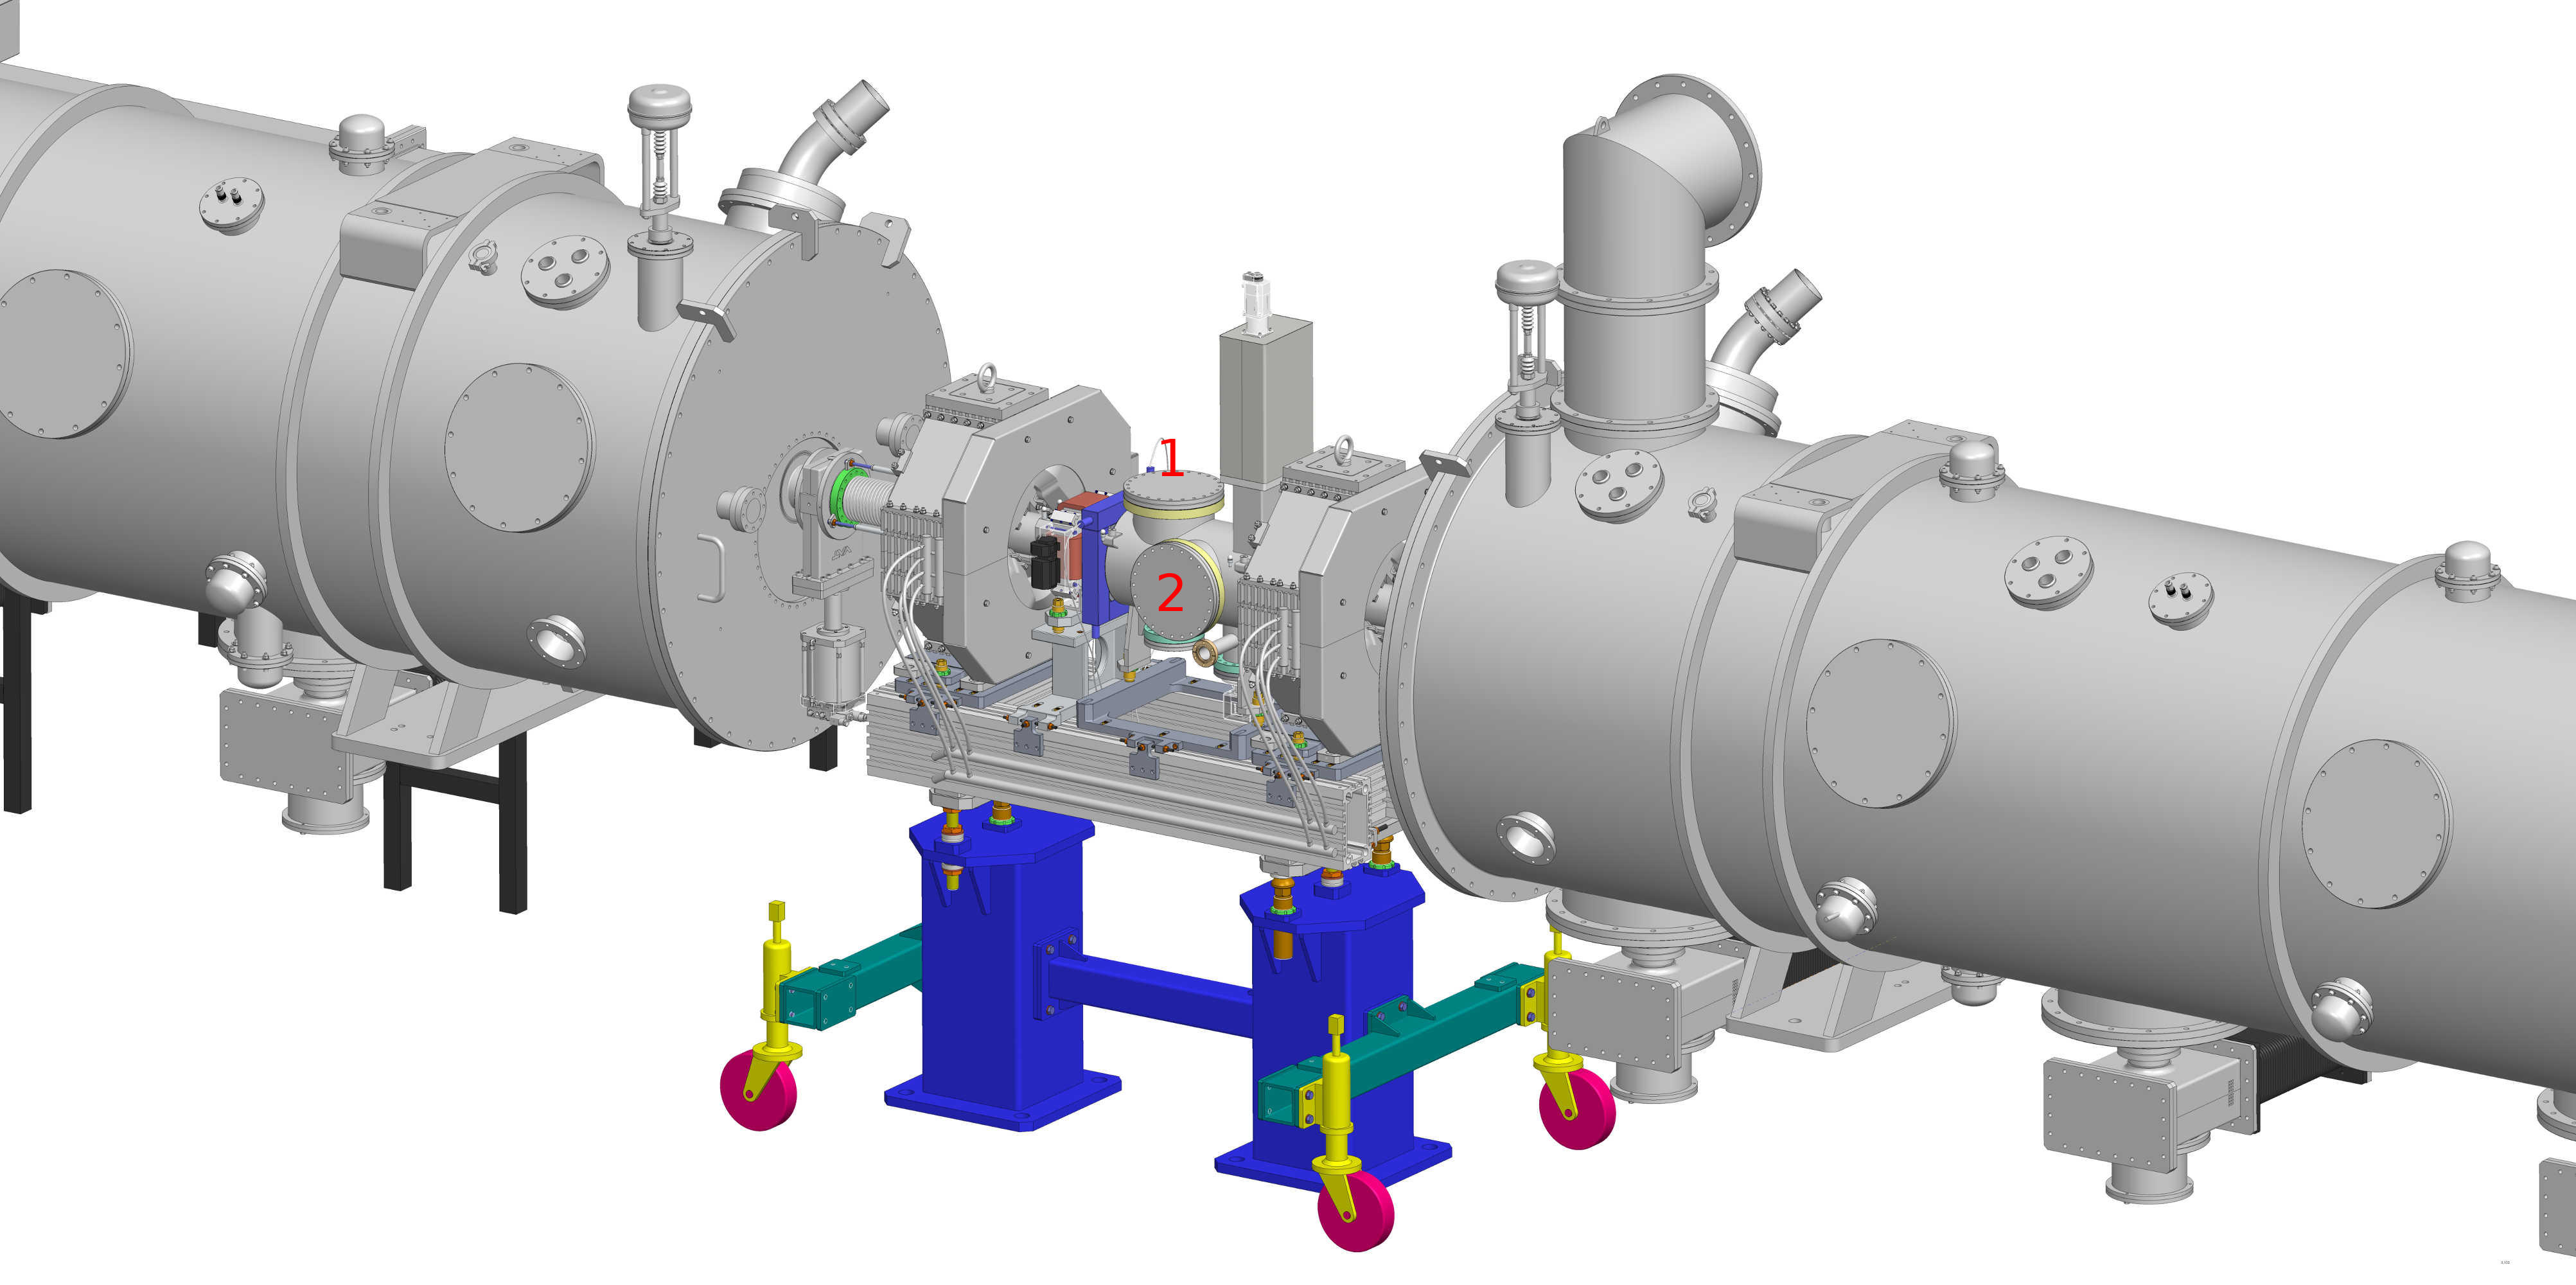
\includegraphics[width=\textwidth]{03_Prototype/figures/fig016_LWU_Cryo3.jpeg}
	\caption[The LWU vessel located between two quadrupole magnets and two cryomodules]{The LWU vessel located between two quadrupole magnets and two cryomodules. The IPMs will be mounted on the CF 200 flanges 1 and 2.}
	\label{chap3:LWU_Cryo}
\end{figure}


  The \acrshort{ipm}s will be located between two cryomodules in the cold accelerator area. The \acrshort{lwu} vessels are not cooled down, but their proximity to the superconducting cavities imposes a high vacuum level and a clean environment. Indeed, a too high pressure or a contamination may damage the cavities. An operating pressure of \(10^{-9}\,\mathrm{mbar}\) is foreseen, but the vacuum level may be even lower during the operation. Safety valves will be closed in case of the vacuum reaches \(10^{-7}\,\mathrm{mbar}\). Hence, quantitatively the \acrshort{ipm} design must be compliant with a high to ultra high vacuum level and an ISO-5 \cite{ISO14644} particle-free environment. Fig. \ref{chap3:LWU_Cryo} shows the \acrshort{lwu} vessel located between two cryomodules. One can see the two \acrshort{cf} 200 flanges devoted to X and Y \acrshort{ipm}s and the two rectangular \acrshort{cf} flanges for the X and Y wire scanners.

  \section{IPM simulations overview}

  \begin{wrapfigure}{r}{0.5\textwidth}
	\centering
	\begin{tikzpicture}%[scale=1.3]
		% Variables
		% Ipm
		\pgfmathsetmacro{\LIPM}{1.8};
		\pgfmathsetmacro{\HIPM}{1.8};
		\pgfmathsetmacro{\TIPM}{0.1};
		% Deg
		\pgfmathsetmacro{\LDEG}{0.1};
		\pgfmathsetmacro{\HDEG}{0.3};
		\pgfmathsetmacro{\NDEG}{6};
		\pgfmathsetmacro{\SDEG}{1.5};
		\pgfmathsetmacro{\SPAND}{(2*\SDEG - \HDEG)/\NDEG}

		\draw[] (\LIPM,0) node[right,align=left] {Field\\correctors\\or\\degraders};


		% Beam
		\draw[fill=blue!30] (0,0) circle (0.4) node[left,xshift = -0.3cm] {Beam};
		% Cage
		\draw (0,0) (-\LIPM,\HIPM)rectangle(\LIPM,\HIPM+\TIPM) node[above] {Anode};
		\draw (0,0) (-\LIPM,-\HIPM)rectangle(\LIPM,-\HIPM-\TIPM) node[below] {Cathode};
		\draw[fill=red!50] (-\LIPM/2,-\HIPM) rectangle(\LIPM/2,-\HIPM-\TIPM) node[midway,below] {Readout};
		% Ionized particle
		\draw[blue, dashed,->] (0.1,0.8)--(0.1,\LIPM);
		\draw[blue,fill=blue] (0.1,0.8) circle [radius=1mm] node[] {\tiny\color{white}{$-$}};

		\draw[red, dashed,->] (0.16,-1)--(0.16,-\LIPM);
		\draw[red,fill=red] (0.16,-1) circle [radius=1mm] node[] {\tiny\color{white}{$+$}};

		\draw[blue,dashed,->] (-0.1,0.1)--(-0.1,\LIPM);
		\draw[blue,fill=blue] (-0.1,0.1) circle [radius=1mm] node[] {\tiny\color{white}{$-$}};

		\draw[red,dashed,->] (-0.1,-0.1)--(-0.1,-\LIPM);
		\draw[red,fill=red] (-0.1,-0.1) circle [radius=1mm] node[] {\tiny\color{white}{$+$}};

		%Field
		\draw[->] (-1.2,1.5)--(-1.2,0.6) node [midway,right]{$\vec{E}$};
		% Degradors
		\foreach \x in {0,...,\NDEG}{
				\draw (0,0) (-\LIPM,\x*\SPAND - \SDEG) rectangle (-\LIPM+\LDEG,\x*\SPAND+\HDEG-\SDEG);
				\draw (0,0) (\LIPM,\x*\SPAND - \SDEG) rectangle (\LIPM-\LDEG,\x*\SPAND+ \HDEG-\SDEG);}


		%Profile
		\begin{axis}[every axis plot post/.append style={
						mark=none,domain=-3:3,samples=50,smooth},
				clip=false,
				axis y line=none,
				axis x line*=bottom,
				ymin=0,
				ymax=1,
				xtick=\empty,
				width=4cm,
				height=3cm,
				scale only axis,
				xshift=-2cm,
				yshift=-3.5cm
			]
			\addplot {\gauss{0}{0.3}{0.3}};
		\end{axis}

	\end{tikzpicture}
	\centering
	\caption[Visual explanation of how an IPM works]{Visual explanation of how an IPM works. The electric field between the electrodes can be reverted by inverting the polarity, making it possible to choose if detecting ions or electrons. Field correctors or degradors, left and right, improve the field uniformity.}
	\label{chap3:ipm_outline}
\end{wrapfigure}


  As explained in the previous chapter, an Ionization Profile Monitor (\acrshort{ipm}) is a non-invasive detector (\acrshort{npm}) that measures the transverse profile of a beam.
  Its principle of operation is shown in Fig. \ref{chap3:ipm_outline} and can be summarized in 3 main steps:
  \begin{enumerate}
    \item Beam protons pass through the vacuum, inducing ionizations of the residual gas molecules: electron/ion pairs are created.
    \item Inside the \acrshort{ipm}, a strong electric field drives electrons or ions towards a segmented readout system.
    \item The profile is reconstructed in one transverse direction. For a complete profile, a pair of \acrshort{ipm}s, rotated by $90\textdegree{}$ with respect to each other, is mandatory.
  \end{enumerate}

  Unfortunately, there is no software that allows a full simulation of an \acrshort{ipm}. Each step requires specific tools. As a consequence, a non-negligible work is necessary to link together the results obtained by the different steps of the simulations. Each simulation can be split in the 3 main parts, as reported just above. This chapter deals with all the simulations and approximations that have been developed to design our detector.

  It is important to underline that designing \acrshort{ipm}s to work in the requested conditions is really challenging. Preliminary studies were carried out by the NPM team in order to check the feasibility of the \acrshort{ipm} design. The efforts have been focussed on the following hot topics:
  \begin{itemize}
    \item Quantification of the ionization signal in terms of number of produced electron/ion pairs, for ensuring that the signal is sufficiently high for reconstructing a profile per pulse, despite of the low gas pressure and ionization cross section at high proton energy.
    \item The extraction field must be as uniform as possible in order to lead efficiently and correctly the ionization by-products toward the readout. %Difficulties come from the small amount of space available in the \acrshort{lwu}.
    \item The space charge effect induced by the beam and the initial momentum of ionization electrons/ions, which may distort the profile, must be evaluated.
    \item The choice of an efficient readout technology which must match \acrshort{ess} working conditions.
  \end{itemize}
  All these points will be presented in the next sections.

  %  Firstly, the primary number of electron/ion pair created by the proton beam should be evaluated, and it must be sufficient in order to reconstruct a beam profile. However, this does not guaranteed that the primary particles reach the readout plane. Thus, it is necessary to perform some electromagnetic simulations. Indeed, primary particle are sensitive to the non uniformities of the extraction field and to space charge effects induced by the beam. These effects may disturb the profile measurements or reduce the number of primary particles. Therefore, they should be quantified. Lastly, the signal creation in the readout device should be evaluated with respect to previous simulations. The response of the readout mainly depends on its type.

  \section{Particle through matter}
  \label{chap3:sec_particle_in_matter}
  The interactions of particles with matter are an important aspect of particle detection \cite{Knoll2010,Leo1994}. A particle will lose energy when it passes through a medium. The physical process behind the energy transfer mainly depends on the characteristics of the particle and the medium. These topics have been studied and improved over the last century. They often combine complicated theoretical laws with approximations or empirical models. This topic is very wide, hence in the following only the pertinent information for this study will be reported.

  As explained before, the \acrshort{ipm}s rely on the by-product collection of the ionized residual gas. The number of ionized particles gives the signal strength which has to be compliant to the readout sensitivity. Therefore, we need to know how many particles are generated by the beam itself along the residual gas enclosed in the accelerator beam pipe. Then we should understand how these secondary particles create a signal in the sensitive part of our \acrshort{ipm}.


  \subsection{Interaction of charged particles with matter}
  For heavy charged particles, the main interaction is due to electromagnetic interactions of the incident particle with the orbiting electrons of the medium. A particle is considered heavy if its mass is much higher than the mass of an electron. The incident particle transfers a small amount of its energy to an electron of the medium at each electronic collision. In 1930, H. Bethe (original paper \cite{Bethe1930}) proposed an equation that describes the mean rate of energy losses per distance unit by a heavy charged particle. The so-called Bethe equation derives from coulomb interactions. This equation has been improved over years \cite{Fermi1940,Fano1963}. The expression of the linear stopping power for heavy charged particles is defined by the following equation \cite[p. 446]{Tanabashi2018}:
  \begin{equation}
    - \bigg \langle \frac{dE}{dx} \bigg \rangle =K \rho \frac{Z}{A} \frac{z^{2}}{\beta^{2}} \left[\frac{1}{2} ln \left(\frac{2 m_{e} \beta^{2} \gamma^{2} T_{max}c^{2}}{I^{2}} \right) - \beta^{2} - \frac{\delta(\beta \gamma)}{2} - \frac{C}{Z} \right]
  \end{equation}
  \noindent where \(K\) is a constant factor defined by \(K=4 \pi N_{a} r_{e}^{2} m_{e} c^{2}\), \(r_{e}\) is the classical electron radius, \(m_{e}\) is the electron mass, \(N_{a}\) the Avogadro constant and $c$ the speed of light in vacuum. For convenience, the stopping power is usually expressed in \(\mathrm{MeV/cm}\). In this case, \(K\) is equal to \(0.307075\,\mathrm{MeV \, mol^{-1} \, cm^{2}}\).

  Terms in the Bethe equation can be dissociated in two groups. First, the incident particle related terms. The maximum transfer energy for one collision is given by the following equation:
  \begin{equation}
    T_{max} = \frac{2 m_{e} \beta^{2} \gamma^{2} c^{2}}{1 + \frac{2 \gamma m_{e} }{M} + \left( \frac{m_{e}}{M} \right)^{2}}
  \end{equation}
  \noindent where, \(M\) and \(m_{e}\) are respectively the incident particle and electron masses. The \(\beta\) and \(\gamma\) variables have their normal significance as Lorentz factors.

  Finally, the terms related to the medium, \(Z\), \(A\) and \(\rho\) are respectively the atomic number, the mass number and the density of the given medium. In most of the cases the \(\frac{Z}{A}\) ratio is close to \(0.5\) except when a medium contains hydrogen. Sometimes, the Bethe equation is given independently from the density.
  The mean excitation energy \(I\) is the only non-trivial variable in the Bethe equation \cite{Berger1984,Berger1993}. The computation is quite complicated because it requires to measure the oscillator strength for each material. Table \ref{chap3:WandI} gives the \(I\) value for common materials.

  Two correction factors are often used to improve the accuracy of the Bethe equation at low and high energies. The term \(\frac{1}{2}\delta(\beta \gamma)\) corrects for the density effects at relativistic energies \cite{Sternheimer1984}. The shell correction \(\frac{C}{Z}\) improves the accuracy at low energies \cite{Bichsel2002}.

  \begin{figure}[!ht]
	\includesvg[width=\textwidth]{03_Prototype/figures/fig001_bethe_4}
	\caption[Typical mass stopping power plot a proton]{Typical mass stopping power plot for a proton. Here the mass stopping power is plotted for a proton in hydrogen and nitrogen. The calculation was done using the Bethe formula and has been cross-checked with the NIST PSTAR table which contains both computed and experimental values \cite{Seltzer1993}.}% The Bethe %equation gives correct results between \(0.2\ <\ \beta\gamma\ <\ 100\). %However at lower and higher energies the Bethe formula is no more reliable.}
	\label{chap3:bethe1}
\end{figure}


  Fig. \ref{chap3:bethe1} shows the mass stopping power of a proton in two different media. The blue region represents the energy range of protons in the cryogenic part of \acrshort{ess}, where \acrshort{ipm}s will be located. One can see that the minimum of energy loss is reached around \(2\,\mathrm{GeV}\).

  The Bethe model has been tested and improved with respect to experimental data \cite{Porter1990}. However, at very low or high energies\footnote{Below $\mathrm{MeV}$ and above hundred $\mathrm{GeV}$ for protons.} the Bethe equation is no more usable. In these regions specific models are used to describe the energy loss in matter \cite{Ziegler1985, Allison1980}.

  The Bethe model is also not compatible with low mass particles like electrons and positrons and must be modified for these particles \cite{Rieke1972}\cite[p. 452]{Tanabashi2018}. At low energies, electrons lose their energies by ionization like ions, whereas at energies above few \(\mathrm{MeV}\), electrons also lose energy through bremsstrahlung radiation.

  \subsection{Electron ion pairs production}
  We just defined the mean energy loss rate of a charged particle per unit of distance. When a particle passes through a medium, it may transfer its energy to the medium, which for now we consider as composed of atoms not bound in molecules. If the energy is sufficient, an ionization happens: one or more electrons are ejected from the electronic shells, leading to the creation of an ion and free electron(s). In case of molecules, the ionization process may be dissociative i.e. it may break the molecular bounds. The cross section for dissociative ionization is far lower than the one for pure ionization \cite{Dimopoulou2004}.

  By introducing \(W\), the average energy for producing an ion/electron pair in a medium, we can estimate the number of ion/electron pairs created in a given readout length $\Delta x$ of materials \cite{Weiss1955,Bichsel1979} as:

  \begin{equation}
    N_{electrons}= \frac{\big \langle \frac{dE}{dx} \big \rangle}{W} \Delta x
  \end{equation}

  When an electron is ejected, it has a certain probability for ionizing other atoms if its energy is high enough. These secondary electrons are called delta rays or delta electrons. This phenomenon becomes rare and negligible when the medium has a very low density like in a vacuum system. The \(W\) parameter includes the delta ray electrons, hence the \(W\) value is biased \cite[p. 470]{Tanabashi2018} for the case at hand, since the \acrshort{ipm}s work at very low pressure. Table \ref{chap3:WandI} gives, as an example, the \(W\) values for several materials at Normal Temperature and Pressure\footnote{$20\,\mathrm{°C}$, $1\,\mathrm{atm}$.} (NTP).

  \begin{table}[ht]
	\centering
	\caption[Mean excitation energie, average energy to produce a pair and density values for severals mediums at Normal Temperature and Pressure (NTP)]
	{Mean excitation energie, average energy to produce a pair and density values for severals mediums at Normal Temperature and Pressure (NTP). Complete reviews of \(I\) and \(W\) values are available in \cite{Kamakura2006}\cite{Bichsel1979}.}
	\label{chap3:WandI}
	\begin{tabular}{llll}
		\toprule
		Gas        & \(I\) (\(\mathrm{eV}\)) & \(W\) (\(\mathrm{eV}\)) & \(\rho\) (\(\mathrm{kg/m^{3}}\)) \\
		\midrule
		\(H_{2}\)  & \(18.8\)       & \(36.43\)  &  \(0.0899\)  \\
		\(CO\)     & \(85.9\)       & \(34.5\)   &  \(1.165\)  \\
		\(CO_{2}\) & \(85.00\)      & \(34.21\)  &  \(1.842\)  \\
		\(N_{2}\)  & \(82.00\)      & \(36.39\)  &  \(1.165\)  \\
		\bottomrule
	\end{tabular}
\end{table}

  When the medium is a mixture of several compounds, its mean stopping power needs to be calculated as the sum of the mean stopping power of its components weighted by their mass proportion. As a consequence, the total number $N_{total}$ of electron/ion pairs results:
  \begin{equation}
    N_{total}= \sum_{n= First}^{Last} N_{compound}= \sum_{n= First}^{Last} w_{n} \frac{\big \langle \frac{dE}{dx}\left(\rho_{n},I_{n},A_{n},Z_{n}\right) \big \rangle}{W_{n}} \Delta x
  \end{equation}
  The calculation can be done for each single element or for each molecule in the compound.
  This latter is recommended since the \(I\) values are in general higher for molecules \cite[p. 451]{Tanabashi2018}.

  \subsection{Calculation}
  \label{chap3:calc}
  Following the physics introduction reported above, this subsection is dedicated to the estimation of the number of primary particles that will be created at the \acrshort{ess} conditions. Two different approaches have been done: naive computation of Bethe equation and simulations through a software.

  The Bethe formula can be implemented in a spreadsheet or a C++ code once the composition of the medium and the \(I\) value of each compound is known. The expected pressure in the cryogenic part at \acrshort{ess} is around \(10^{-9}\,\mathrm{mbar}\), and the gas composition is given in Table \ref{chap3:ess_vacuum_gas}.

  \begin{table}[ht]
	\centering
	\caption[Expected residual vacuum gas in the cold part of ESS Linac, provided by ESS vacuum group]
	{Expected residual vacuum gas in the cold part of ESS Linac, provided by ESS vacuum group.}
	\label{chap3:ess_vacuum_gas}
	\begin{tabular}{llll}
		\toprule
		Gas        & Mass percentage (\(\%)\) & $p_{i}$ (\(\mathrm{mbar}\)) & $\rho_{i}$ $(\mathrm{g/cm^{3}}$) \\
		\midrule
		\(H_{2}\)  & \(79\)          & \(7.9 10^{-10}\)   & \(6.52\cdot
		10^{-17}\)                                                                \\
		\(CO\)     & \(10\)          & \(1.0 10^{-10}\)   & \(1.15\cdot
		10^{-16}\)                                                                \\
		\(CO_{2}\) & \(10\)          & \(1.0 10^{-10}\)   & \(1.8\cdot
		10^{-16}\)                                                                \\
		\(N_{2}\)  & \(1\)           & \(1 10^{-11}\)     & \(1.14\cdot
		10^{-17}\)                                                                \\
		\bottomrule
	\end{tabular}
\end{table}

  We assume that the residual gas follows the "perfect gas" law. We also assume that the linear density scaling of Bethe equation remains true in high vacuum \cite[p. 108]{egberts2012}\cite{Ishimaru1995}. Hence, the partial pressure and the density for each gas is calculated with respect to the tabulated pressures. The primary signal is computed at \acrshort{ess} nominal conditions given in Table \ref{chap2:tab:ess_charac}.

  Fig. \ref{chap3:ess_primary_particles} shows the number of electron ion pairs created for each gas species versus the \acrshort{ess} proton beam energy. The different \acrshort{ipm}s locations are marked by a blue line. One can see that the gas density has a strong influence on the primary signal. Although the hydrogen is the main species in terms of proportion, its contribution to the signal is close to the one from carbonate species. Note that the \(W\) value may overestimate the number of pairs created due to secondary delta rays.
  \begin{figure}[!ht]
	\includesvg[width=\textwidth]{03_Prototype/figures/fig015_ess_primary_particle}
	\caption[Expected number of electron/ion pairs per centimeter at ESS nominal conditions according to Bethe equation]{Expected number of electron/ion pairs per centimeter at ESS nominal conditions according to Bethe equation. Each vertical line corresponds to an IPM location.}
	\label{chap3:ess_primary_particles}
\end{figure}


  We have also used the Garfield++ software to compute the number of primary  ionizations. This software is normally intended for the modelization of gaseous detectors. It allows to simulate the creation of electron/ion pairs due to the ionization of gas by an incident particle, the transport and amplification of these electrons in the gas and the signal induced on a readout plane. In our case, we simulated only the pair creation in the residual gas. For this step Garfield++ uses two programs internally:
  \begin{itemize}
    \item Magboltz: a Fortran routine that computes different properties of a gas mixture and performs the transport of electrons in this mixture \cite{Biagi1989}.
    \item Heed ++ \cite{Smirnov2005}: a C ++ code that implements an ionization model based on the photoabsorption ionization (PAI) \cite{Allison1980}.
  \end{itemize}

  \begin{table}[ht]%{r}{0.5\textwidth}
	\centering
	\caption[Comparison of expected number of electrons between calculation using Bethe equation and results from Garfield++.]
	{Comparison of expected number of electrons between calculation using Bethe equation and results from Garfield++}
	\label{chap3:GarfieldBethe}
	\begin{tabular}{llll}
		\toprule
		Energy    & \(N_{Bethe}\) & \(N_{garfield}\) & Factor \\
		\midrule
		\(97.2\)  & \(100210\)    & \(52537\)             & \(0.52\)   \\
		\(231.4\) & \(54970\)     & \(27463\)             & \(0.50\)   \\
		\(278.9\) & \(49160\)     & \(26124\)             & \(0.53\)   \\
		\(315.8\) & \(45850\)     & \(23769\)             & \(0.52\)   \\
		\(628.3\) & \(33600\)     & \(17522\)             & \(0.52\)   \\
		\bottomrule
	\end{tabular}
\end{table}
  A dummy detector, a cube of ten centimeter side, is implemented and filled with the same gas composition as in Table \ref{chap3:ess_vacuum_gas}. Protons are shot into this detector and the information on the electrons created in the gas is saved in a ROOT file \cite{Brun1997,Antcheva2009} for post processing. This is done for different proton energies and vacuum levels.

  Table \ref{chap3:GarfieldBethe} reports the value of the expected number of electrons/ions pairs per cm obtained from the direct calculation (Bethe equation) and from the results of the Garfield++ simulations. One can see that the Garfield++ value is always lower than the calculation by a constant factor $0.52$. These value are important since they will be used to determine the readout technology and its electronics. 

  \subsection{Pressure uniformity}
  The primary signal is strongly dependent on the pressure inside the vacuum chamber. A gradient in the pressure may cause a change in the signal shape. It is therefore interesting to simulate the vacuum level in the \acrshort{lwu} to check the existence of such gradient in the residual gas of the \acrshort{ipm}s.

  \begin{wrapfigure}{r}{0.5\textwidth}
  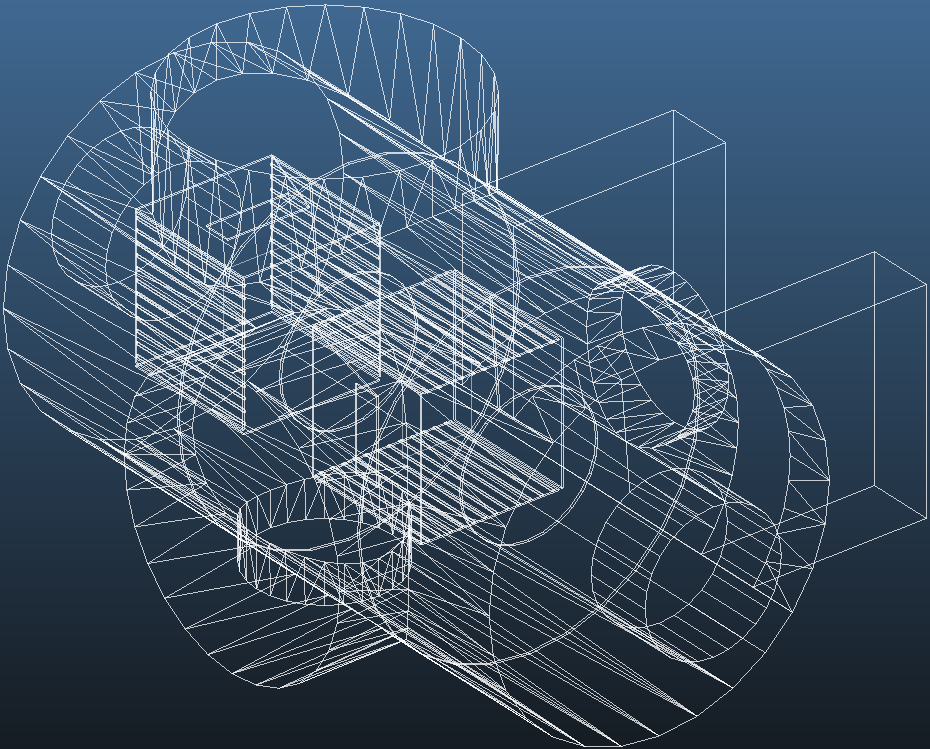
\includegraphics[width=0.5\textwidth]{03_Prototype/figures/fig019_molflow_LWU.png}
  \caption[The LWU geometry implemented in Molflow+]{The LWU geometry implemented in Molflow+.}    
	\label{chap3:molflow_LWU}
\end{wrapfigure}

  A simulation has been done with the Molflow+ software developed at CERN \cite{Kersevan2009}. It simulates the vacuum in a steady state by using Monte Carlo and Ray Tracing methods. The user defines his geometry, as well as the desorption and adsorption rates of each surface. As visible in Fig. \ref{chap3:molflow_LWU}, the implemented geometry does not contain all the structures and surfaces. Two dummy squared facets of $5\,\mathrm{cm}$ side are inserted in the center of each \acrshort{ipm}. The pressure profiles are then measured on these facets. No information about the real pumping speed, surface conditions or other vacuum characteristics is input in the program since the only goal of this simulation is for checking the non-uniformity effect of the residual gas pressure for both \acrshort{ipm}s. We have also checked the case of an unwanted outgassing which may occur on one side of the \acrshort{ipm}s. No significant change has been observed.

  Fig. \ref{chap3:profile_pressure} shows the results from the simulations. The pressure levels seem to be uniform for both \acrshort{ipm}s along the transverse direction, and it may not affect the profile measurement. The pressure is slightly lower in the second \acrshort{ipm} because the pumping group is closer.

  \begin{figure}[!h]
	\begin{center}
		\includesvg[width=\textwidth]{03_Prototype/figures/fig020_profile_pressure}
	\end{center}
	\caption[Simulated profile pressure in the center of IPMs.]{Simulated profile pressure in the center of IPMs.}
	\label{chap3:profile_pressure}
\end{figure}

  \FloatBarrier
  \section{Extraction field}
  \begin{wrapfigure}{r}{0.5\textwidth}
	\centering
	\begin{tikzpicture}
		% Variables
		% Ipm
		\pgfmathsetmacro{\LIPM}{1.8};
		\pgfmathsetmacro{\HIPM}{1.8};
		\pgfmathsetmacro{\TIPM}{0.1};
		% Deg
		\pgfmathsetmacro{\LDEG}{0.1};
		\pgfmathsetmacro{\HDEG}{0.3};
		\pgfmathsetmacro{\NDEG}{6};
		\pgfmathsetmacro{\SDEG}{1.5};
		\pgfmathsetmacro{\SPAND}{(2*\SDEG - \HDEG)/\NDEG}

		% Beam
		\draw[fill=blue!30] (0,0) circle (0.4) node[left,xshift = -0.3cm] {Beam};
		% Cage
		\draw (0,0) (-\LIPM,\HIPM)rectangle(\LIPM,\HIPM+\TIPM) node[above] {Anode};
		\draw (0,0) (-\LIPM,-\HIPM)rectangle(\LIPM,-\HIPM-\TIPM) node[below] {Cathode};
		\draw[fill=red!50] (-\LIPM/2,-\HIPM) rectangle(\LIPM/2,-\HIPM-\TIPM) node[midway,below] {Readout};
		% Ionized particle
		\draw[blue, dashed,->] (0.1,0.8)to [bend right=15](-0.1,\LIPM);
		\draw[blue,fill=blue] (0.1,0.8) circle [radius=1mm] node[] {\tiny\color{white}{$-$}};

		\draw[red, dashed,->] (0.36,-1)to [bend left=0](0.56,-\LIPM);
		\draw[red,fill=red] (0.36,-1) circle [radius=1mm] node[] {\tiny\color{white}{$+$}};

		\draw[blue,dashed,->] (-0.1,0.1)to [bend right=15](-0.8,\LIPM);
		\draw[blue,fill=blue] (-0.1,0.1) circle [radius=1mm] node[] {\tiny\color{white}{$-$}};

		\draw[red,dashed,->] (-0.1,-0.1)to [bend right=15](0.2,-\LIPM);
		\draw[red,fill=red] (-0.1,-0.1) circle [radius=1mm] node[] {\tiny\color{white}{$+$}};

		%Field
		\draw[->] (-1.2,1.5)--(-1,0.6) node [midway,right]{$\vec{E}$};

		% Profile
		\begin{axis}[every axis plot post/.append style={
						mark=none,domain=-3:3,samples=50,smooth},
				clip=false,
				axis y line=none,
				axis x line*=bottom,
				ymin=0,
				ymax=1,
				xtick=\empty,
				width=4cm,
				height=3cm,
				scale only axis,
				xshift=-2cm,
				yshift=-3.5cm
			]
			\addplot {\gauss{0.75}{0.5}{0.3}};
		\end{axis}
	\end{tikzpicture}
	\centering
	\caption[Non-uniformities leading to mirage effects on the profile measurement]{Non-uniformities leading to mirage effects on the profile measurement.}
	\label{chap3:FieldNonU_outline}
\end{wrapfigure}

  The \acrshort{ipm}s can be seen as parallel plate detectors. In an ideal \acrshort{ipm} these plates are infinite sized. The extraction field is then completely oriented in a single direction, normal to the detection plane and the projection of the profile on this plane is perfect. In reality, the plates have finite dimensions, comparable to the gap between the two electrodes. In these conditions the field is no longer uniform.

  The effects induced by the cage sides are no longer negligible; field uniformity is strongly influenced by the needle effects of the plates.
  Also, the geometry of the vacuum chamber affects the field uniformity: it is considered to be at ground but walls close to the \acrshort{ipm}s modify the electric field lines inside the \acrshort{ipm}s. In addition, the cross-interaction between the electric fields of two close by \acrshort{ipm}s is very strong.

  Finally, the way to create the field with high voltage (\acrshort{hv}) power supplies has an important influence on the electric field itself. We will see later that some readouts can only work in certain HV configurations, unless major modifications of the set-up are considered.

  The non-uniformity of the electric field is very problematic because it creates distortion effects and prevents the correct measurement of the beam profile as shown in Fig. \ref{chap3:FieldNonU_outline}. It also determines the maximum size of the detection area, which must be in a zone where the electric field is as uniform as possible. To overcome the distortion effect, the field line must be as straight as possible. Several solutions can be considered to improve the field uniformity:
  \begin{itemize}
    \item The distance between the two electrodes can be reduced. In this case, the \acrshort{ipm}s will tend to a configuration close to the infinite parallel plates assumption. Following the same logic, the size of both electrodes could be increased. These solutions are mainly limited due to mechanical considerations. To stay on the safe side, the distance between two plates was chosen to be at least equal to the diameter of the beam pipe. Moreover, the whole assembly of one \acrshort{ipm} must hold on a CF 200 flange.
    \item Using field correctors or field degraders \cite[p. 103]{egberts2012}. This is done by placing conductors on each side. Each corrector is set to a certain potential in order to constrain the field. This solution is easy to implement, compact, and very versatile. However, it requires a large number of \acrshort{hv} feedthroughs or the use of resistors in vacuum. The longitudinal field can also be slightly improved in a same way.
    \item Inserting grounded conductors between the two \acrshort{ipm}s \cite[p. 132]{egberts2012} to protect against the \acrshort{ipm} cross-interaction. The longitudinal correctors also reduced the cross-interaction.
    \item Optimizing the geometry of \acrshort{hv} electrodes. For example, with a curved geometry with reinforcements on the edges it is possible to correct the field transversely and longitudinally. Hence, "there is no more need of field correctors" as said in \cite{Bartkoski2014}.
  \end{itemize}
  Aside the above listed solutions, software corrections may be a way to correct the non uniformities. However, as previously explained the non-uniformity of the extraction field is not the only phenomenon responsible for the distortions of the measured profile. It is therefore extremely difficult to implement it, because it requires a perfect mapping of the extraction field to decouple it from other phenomena. Physical corrections are simpler to implement.

  % The second limitation concerns possible \acrshort{hv} breakdowns. In very high vacuum a distance of some millimeter is sufficient to isolate several tens of kilovolts. However, the breakdowns are also strongly influenced by the surface states of the electrodes, the composition of the vacuum and the presence of leakage current \cite{Latham1995}. Hence, we should keep a standoff distance between the electrode and the vacuum vessel (less than 1kV/cm between the \acrshort{ipm}s and \acrshort{lwu}).

  \subsection{Maxwell equations at steady state}
  \label{chap3:sec:maxwell}
  Electric and magnetic fields are perfectly described by the Maxwell's equations. Since we are in vacuum, the Maxwell's equations can be reduced to:
  \begin{alignat*}{3}
    \overrightarrow{\nabla} \cdot \overrightarrow{E}  & = \frac{\rho}{\epsilon_{0}}\quad                                           &  & \text{(Maxwell-Gauss's Law)}   \\
    \overrightarrow{\nabla} \times \overrightarrow{E} & = - \frac{\partial \overrightarrow{B}}{\partial t}\quad                    &  & \text{(Maxwell-Faraday's Law)} \\
    \overrightarrow{\nabla} \cdot \overrightarrow{B}  & = 0\quad                                                                   &  & \text{(Maxwell-Thomson's Law)} \\
    \overrightarrow{\nabla} \times \overrightarrow{B} & = \overrightarrow{J} + \frac{\partial \overrightarrow{E}}{\partial t}\quad &  & \text{(Maxwell-Ampère's Law)}
  \end{alignat*}

  The time derivatives cancel when the field variations over time are negligible compared to the studied phenomena. So, the coupling effects between the electric and the magnetic fields disappear. Therefore, the electrostatic field depends only on the Gauss’s law. In electrostatic, it is quite convenient to introduce the electric potential:
  \begin{equation}
    \vec{E} = - \vec{\nabla}V
  \end{equation}

  \subsection{Solving Poisson's equation}
  The electric potential follows the Poisson's equation:
  \begin{equation}
    \vec{\nabla}^{2}V = -\frac{\rho}{\epsilon_{0}}
  \end{equation}
  or in a more generic notation:
  \begin{equation}
    \Delta v = f
  \end{equation}
  with $f$ the right hand side function.

  The solution of this equation can be found analytically, by relying on the use of complex numbers or Laplace transforms. However, when the size of the problem increases the solution becomes harder to compute, and solving the Poisson's equation on complicated domains is almost impossible. Numerical methods allow to approximate the solutions of partial differential equations (\acrshort{pde}) on non trivial domains. There are many schemes to solve numerically \acrshort{pde}. In this section we will briefly present three methods that are often used. It is important to understand how they work and to know their limitations or pitfalls. In numerical schemes, the domain is discretized in a finite set of points. Then, the solution is approximated at each point with respect to initial and/or boundary conditions. To solve a problem, it must be well posed: the problem must admit a single unique solution that depends continuously on the variables and conditions \cite{Hadamard1902}. It turns out that the Poisson's equation is a well-posed problem if a Dirichlet condition is applied.

  %\paragraph{}
  Finite Difference Method (FDM) is a popular way to solve numerically the Poisson’s equation. In FDM, the domain is discretized regularly with a step $h$. The Taylor's theorem allows to approximate the value of a function by a polynomial equation that depends on its derivatives nearby:
  \begin{align}
     & v(x+h) = v(x)+hv^{\prime}(x)
    +\frac{h^2}{2}v^{\prime\prime}(x)+\frac{h^3}{6}v^{\prime\prime\prime}(x) + O(h^{4}) \\
     & v(x-h) = v(x)-hv^{\prime}(x)
    +\frac{h^2}{2}v^{\prime\prime}(x)-\frac{h^3}{6}v^{\prime\prime\prime}(x) + O(h^{4})
  \end{align}
  From these formulas, the second derivative can be expressed:
  \begin{equation}
    \frac{\partial^{2} v}{\partial x^{2}} = \frac{v(x+h) - 2 v(x) + v(x-h)}{h^{2}} + O(h^{2})
  \end{equation}
  and in case of a two-dimensional domain it is written as follows:
  % h^{2}v^{\prime\prime}(x,y)=
  \begin{equation}
    \begin{split}
      \Delta v & = \frac{\partial^{2} v}{\partial x^{2}} + \frac{\partial^{2} v}{\partial y^{2}} \\
      &= \frac{v(x+h,y) + v(x-h,y)
        + v(x,y+h) + v(x,y-h)
        - 4v(x,y)}{h^2} + O(h^{2})
    \end{split}
  \end{equation}
  Each point of the domain can be expressed according to its neighbors. Then, it is possible to write a set of linear equations in matrix form by choosing wisely the indexing order. For example, when the domain is decomposed line by line, one can obtain the same system of equations repeated for each inner line \footnote{The first and last lines have a slightly different set of equations due to boundary conditions.}.
  \begin{equation}
    Id \cdot v_{u} + A \cdot v_{c} + Id \cdot v_{d} = D
  \end{equation}
  Where $Id$ is the identity matrix, $v_{u}$ are the unknown values of the upper line, $v_{d}$ of the lower line, $v_{c}$ of the current line, $ A =
    \begin{pmatrix}
      -4     & 1      & 0      & \cdots \\
      1      & -4     & 1      & \cdots \\
      0      & 1      & -4     & \cdots \\
      \vdots & \vdots & \vdots & \ddots
    \end{pmatrix} $ is the square matrix of FDM schemes and $D$ is vector of Dirichlet values. Then, the global matrix is assembled by combining the sub-matrices for each line.
  \begin{equation}
    \begin{bmatrix}
      A      & Id     & 0      & \cdots \\
      Id     & A      & Id     & \cdots \\
      0      & Id     & A      & \cdots \\
      \vdots & \vdots & \vdots & \ddots
    \end{bmatrix}
    \cdot
    \begin{bmatrix}
      v \\
      v \\
      v \\
      \cdots
    \end{bmatrix}
    =
    \begin{bmatrix}
      D \\
      D \\
      D \\
      \cdots
    \end{bmatrix}
  \end{equation}
  One can see that the problem is solved by inverting the A matrix. This matrix is very sparse and can be inverted with iterative methods rather than a direct inversion. FDM is straightforward and allows to quickly solve Poisson’s equation on a linear structured mesh. For instance, it is very useful for calculating an electric field generated by a charge density. However, FDM cannot be used when the geometry becomes too complex.

  \paragraph{}
  The Finite Element Method (FEM) is more suitable for solving PDE on complicated domains. The FEM uses the weak formulation of the Poisson’s equation. By introducing a test function $\varphi$, this weak form can be written easily thanks to an integration by parts:
  \begin{align}
    \int_{\Omega}^{} \varphi \Delta v d\Omega                                                                                           & = \int_{\Omega}^{} \varphi f d\Omega \\
    -\int_{\Omega}^{} \vec{\nabla} \varphi \cdot \vec{\nabla} v d\Omega + \int_{\Sigma}^{} \varphi \vec{\nabla} v \cdot \vec{n} d\Sigma & = \int_{\Omega}^{} \varphi f d\Omega
  \end{align}
  with $\Sigma$ the boundary domain.
  One can see that the Laplacian disappeared from the formulation. An approximation of $v$ is done in the reduced domain by means of low order polynomial functions. Again, a finite system of linear equations can be written, and the problem is solved by inverting the matrix. The correct choice of test functions and the way to index elements lead to very sparse matrix which can be inverted easily. Unlike the FDM, the solution is approximated on the whole reduced domain and not locally. FEM supports complicated meshes as long as they are continuous and solves all kinds of PDEs that may be much more complex than the Poisson’s equation.

  \paragraph{}
  % Expliquer mieux les BEM
  With FEM, the whole domain is fully discretized in its entire volume. In case of electrostatic field, it is possible to use the Boundary Element Method (BEM). With the BEM, the Poisson’s equation is first solved on boundaries. Then, the electric field can be evaluated at any point in the domain from the contributions of all boundaries. The discretization is also performed only on the boundaries and not on the entire geometry. So, the dimension of the problem is reduced and the matrix to be reversed is much smaller. On the other hand, the matrix is no longer sparse.

  Most of the commercial simulation softwares \cite{cststudio2018,ansys2018,couloumb2018} rely on FEM or BEM. We have used mainly the COMSOL software for the simulations of extraction fields.

  %jac 1: je trouve que le traitement des FM, BEM et l'autre pourrait être mieux séparés (sous paragraphe ou autre) 

  \subsection{COMSOL}
  COMSOL is a commercial all-in-one multi-physics simulation software able to solve various problems from structural mechanical analysis to optical raytracing \cite{comsol2018}. We used COMSOL with the AC/DC module \cite{comsolacdc2018} to simulate the static electric field in the \acrshort{ipm} box. COMSOL allows to quickly define, simulate and post process physical models. The typical workflow is divided in three main steps as follow.
  \begin{figure}[ht]
	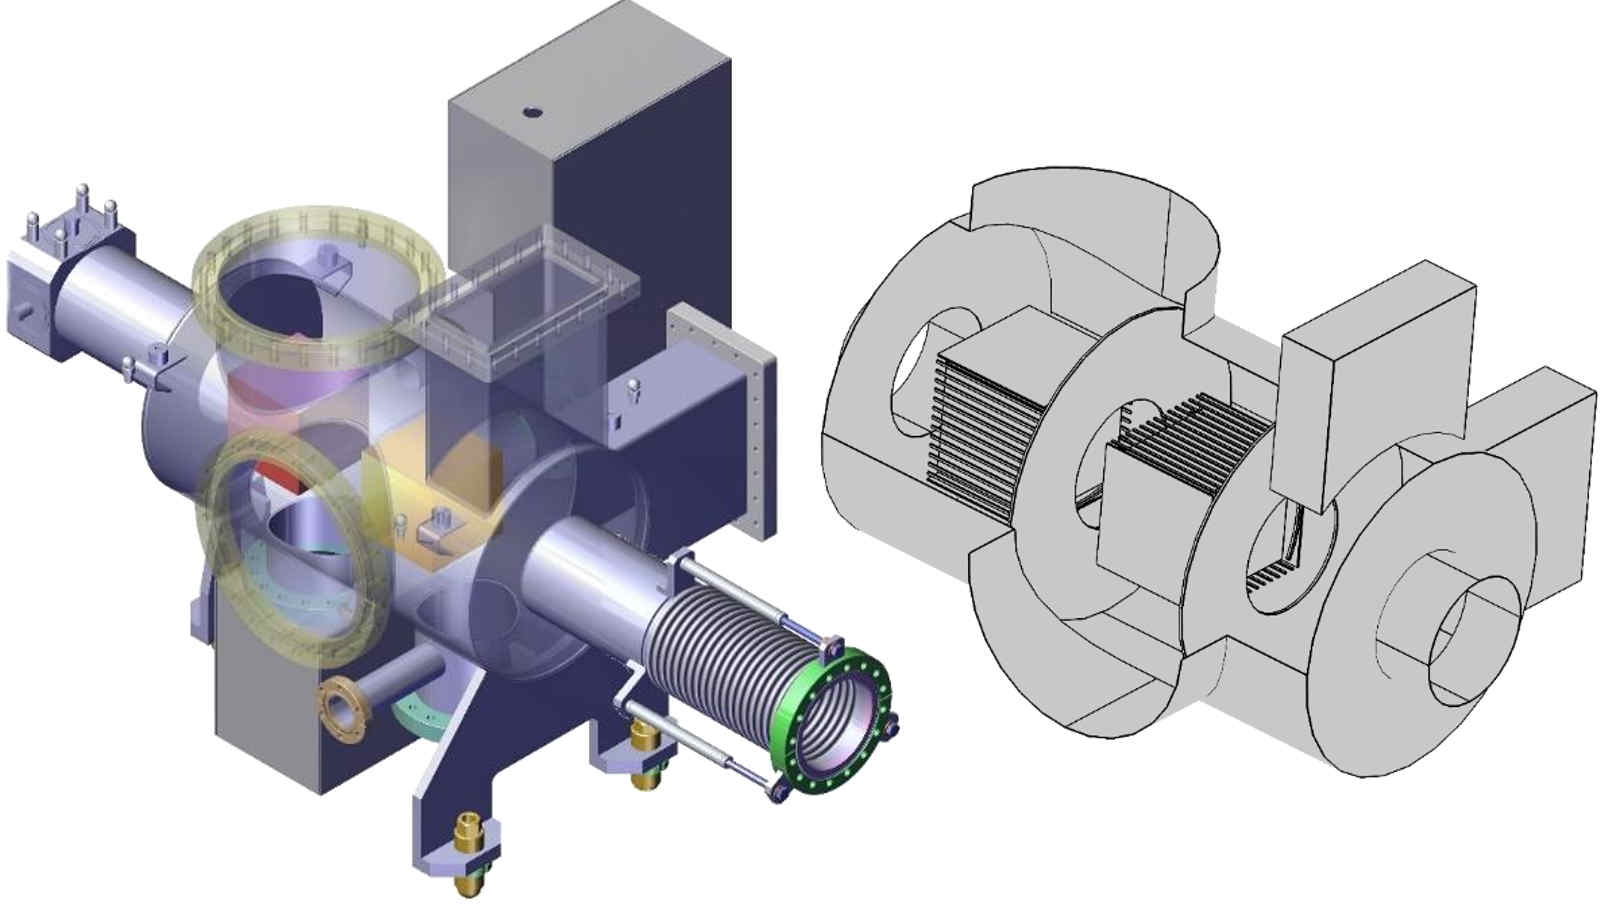
\includegraphics[width=\textwidth]{03_Prototype/figures/fig003_COMSOL_LWU.jpeg}
	\caption[A drawing of LWU (left) and its implementation in COMSOL (right)]{A drawing of LWU (left) and its implementation in COMSOL (right).}
	\label{chap3:COMSOL_LWU}
\end{figure}


  The first step is to implement the detector geometry into COMSOL. The software includes basic \acrshort{cad} features allowing to quickly create two or tridimensional geometries. The users can directly import a mesh from files generated by external \acrshort{cad} tools. Care should be taken for importing a \acrshort{cad} file: it often contains many details and thus increases the CPU time consumption. It is much faster to directly implement the geometry with COMSOL.  In our case, only the inner shape of the vacuum chamber and the \acrshort{ipm}s have been defined. All other conductive bodies that enclose the vacuum are not relevant for an electrostatic simulation. Therefore, the geometry could be simplified. Fig. \ref{chap3:COMSOL_LWU} shows, on the left, a 3D drawing of the \acrshort{ess} vacuum vessel with the two \acrshort{ipm}s inside. And on the right, an example of the simplified geometry implemented in COMSOL.
  \begin{figure}[ht]
	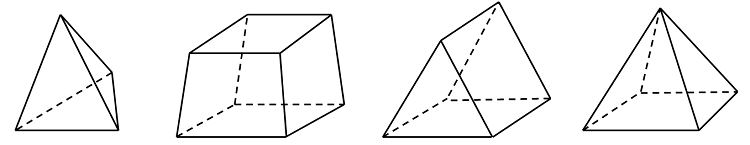
\includegraphics[width=\textwidth]{03_Prototype/figures/fig006_COMSOL_meshing_elements.png}
	\caption[3D Mesh elements included in COMSOL]{Mesh elements included in COMSOL software. From left to right: tetrahedron, hexahedron, prism and pyramid \cite{mesh2013}. COMSOL uses tetrahedral elements by default to mesh a 3D geometry in AC/DC module.}
	\label{chap3:COMSOL_meshing_elements}
\end{figure}


  The next step consists in the discretization of the previous geometry in many Lagrange elements in order to form a mesh. Fig. \ref{chap3:COMSOL_meshing_elements} shows the main meshing elements available in COMSOL. For an electrostatic tri-dimensional study, COMSOL uses quadratic tetrahedral elements by default. The meshing algorithm tries to create elements fitting well the geometry. For the inner small parts of the geometry, the size of elements will be reduced. Conversely, mesh cells will become bigger and bigger in coarse regions of the geometry. This behavior is not desirable for us, since the \acrshort{ipm} region of interest has no geometrical variations. The geometry would not be not described accurately. Fortunately, the user can change the characteristics and the nature of the elements in specific regions of the defined geometry. We used a tetrahedral mesh everywhere but in the \acrshort{ipm} box, where a cubic mesh with high granularity is defined. The meshing step is very memory consuming, but a poorly optimized mesh may destroy performances.
  \begin{figure}[!h]
	\begin{subfigure}{.5\textwidth}
		\centering
		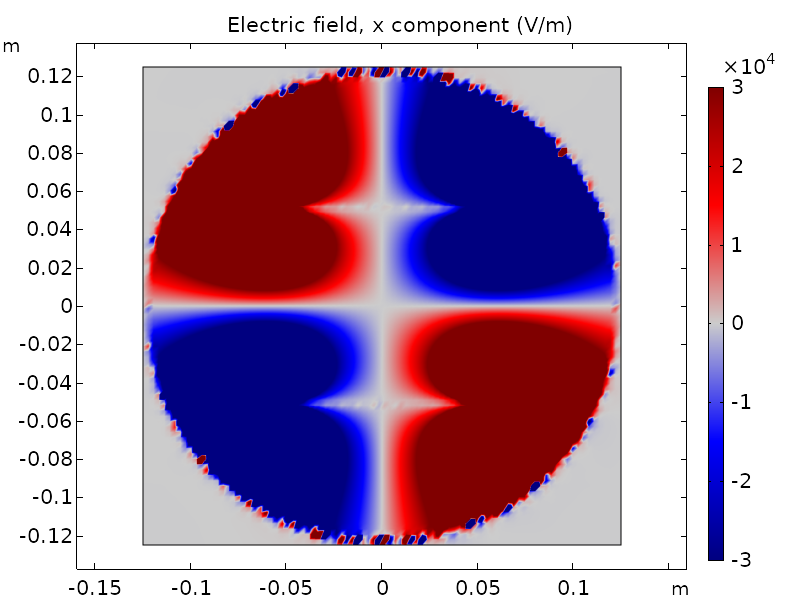
\includegraphics[width=\textwidth]{03_Prototype/figures/fig012_BEMa.png}
		\caption{Configuration 1 solved with BEM.}
		\label{}
	\end{subfigure}\hfill
	\begin{subfigure}{.5\textwidth}
		\centering
		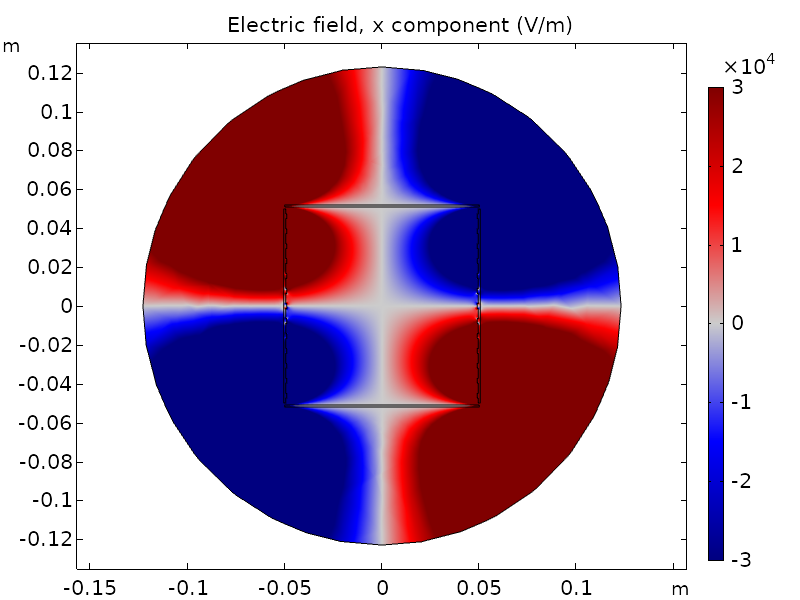
\includegraphics[width=\textwidth]{03_Prototype/figures/fig012_FEMa.png}
		\caption{Configuration 1 solved with FEM.}
		\label{}
	\end{subfigure}
	\vskip\baselineskip
	\begin{subfigure}{.5\textwidth}
		\centering
		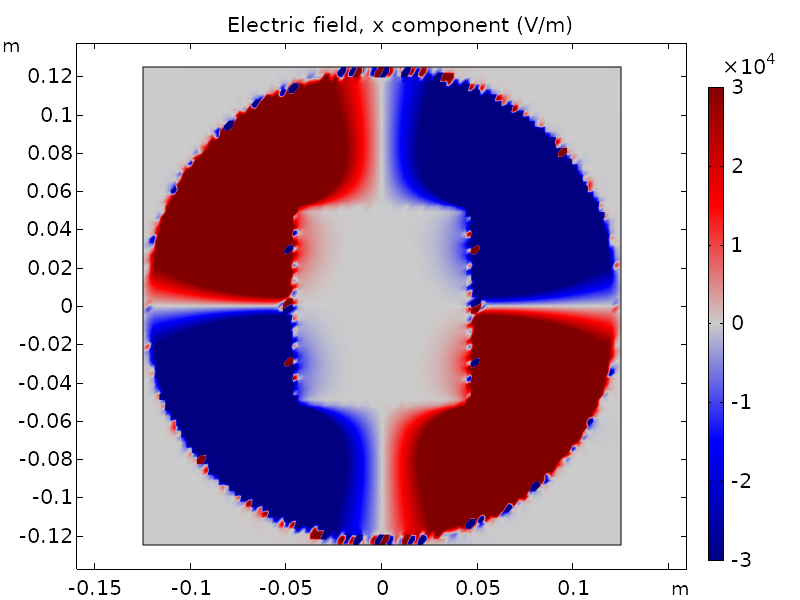
\includegraphics[width=\textwidth]{03_Prototype/figures/fig012_BEMb.png}
		\caption{Configuration 2 solved with BEM.}
		\label{}
	\end{subfigure}\hfill
	\begin{subfigure}{.5\textwidth}
		\centering
		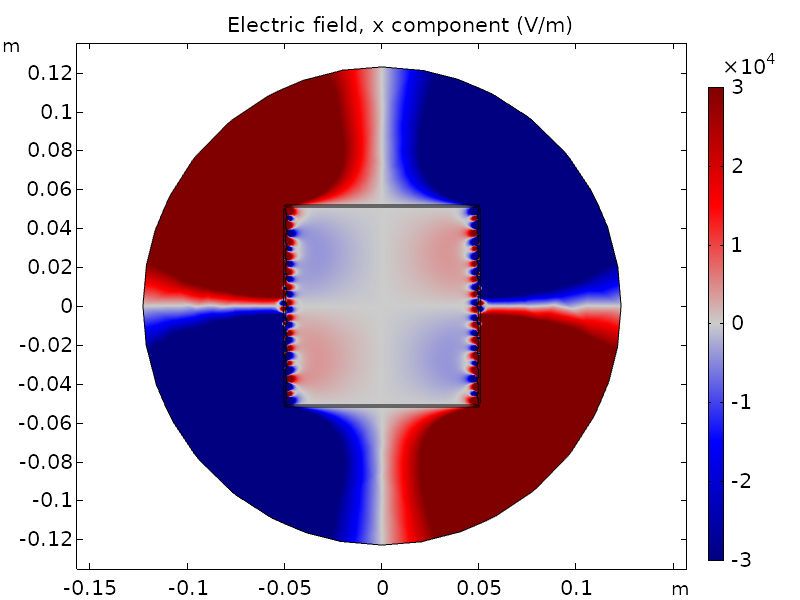
\includegraphics[width=\textwidth]{03_Prototype/figures/fig012_FEMb.png}
		\caption{Configuration 2 solved with FEM.}
		\label{}
	\end{subfigure}
	\caption[Comparison beetwen BEM and FEM for two different IPM configurations]{Comparison beetwen BEM and FEM for two different IPM configurations.}
	\label{chap3:FEMvsBEM}
\end{figure}


  The last step is to define boundary conditions. COMSOL hides completely the mathematical aspect of the \acrshort{fem}/\acrshort{bem} and directly expresses the boundary conditions by associating them a physical meaning. This means that, when using AC/DC module, the user should fix potentials or charge densities on boundaries. A more detailed description of each boundary condition type can be found in the reference manual. COMSOL is able to solve electrostatic problems by means of \acrshort{fem} or \acrshort{bem} since version 5.3a. We compared the \acrshort{fem} and \acrshort{bem} for same configurations and we found out that results are slightly different as shown in Fig. \ref{chap3:FEMvsBEM}. We decided to use mainly \acrshort{fem} since it is the legacy method in COMSOL.
  Once solved, the results can be visualised directly in COMSOL. Data can be also exported to an external file in text format (comma separated values or VTU format).

  Below are listed the relevant assumptions made in our COMSOL model:
  \begin{itemize}
    \item All conductors and insulators are supposed to be perfect.
    \item Field correctors and electrodes are thicker than in reality since it is not feasible to describe a micrometer deposition layer in a meter scale simulation.
    \item Neither the resistor chain at the back of field correctors, nor the connection wires, feedthroughs and connectors are implemented.
    \item The vacuum vessel is supposed to be at the same ground as the power supplies, and without any charge on its surface.
  \end{itemize}

  \subsection{Criteria}
  \label{chap3:sec:criteria}
  It is necessary to define criteria to quantify the uniformity of the electric field in order to compare several simulations. In this thesis, we will use mainly:
  \begin{itemize}
    \item Visual approaches (isocolors and streamlines) that are sufficient at first to underline big differences between two models.
    \item A statistical criterion
    \item Particle tracking
  \end{itemize}
  In this section, we will explain briefly the two last criteria.

  \paragraph{}
  For the statistical criterion, the whole data set is sliced in the longitudinal direction. In each slice, the quadratic mean value of each electric field component is computed in a small cylinder at the center of the \acrshort{ipm}.
  \begin{equation}
    \vec{E}_{mean} = \frac{\sum_{i=1}^{N}\sqrt{\vec{E}_{i}^{2}}}{N}
  \end{equation}
  The only pitfall of this method is the size of the area. The mean value must be computed on an area that covers at least the beam\footnote{We assume that the beam is centered.}. On the other hand, if the area is too big, then the mean value will be biased due to field correctors on each side of the \acrshort{ipm}s.
  To choose the area size, we proceed as follows. A charged particle is released at rest in a dummy \acrshort{ipm} where the field is perfectly uniform, except in a small region. In this region, we add a component perpendicular to the field lines and equal to $1\,\mathrm{\%}$ of the main field value. When the particle reaches the readout, the total deviation is recorded. Then the region is shifted and the computation is repeated. Table \ref{chap3:Deviation} tabulates results.

  \begin{table}[ht]
	\centering
	\caption[Example of deviation of the trajectory of a particle in an IPM]
	{Example of deviation of the trajectory of a particle in an IPM. A particle is released in the center of an IPM with a straight field everywhere, but in a certain range a parasitic field component is added and set to $1\,\mathrm{\%}$ of the main field. The 0 coordinate is the IPM center whereas the readout is at \(5 \, \mathrm{cm}\) distance.}
	\label{chap3:Deviation}
	\begin{tabular}{cccccc}
		\toprule
		                               & \multicolumn{5}{c}{Range (\(\mathrm{cm}\))}                                                 \\
		\cmidrule(lr){2-6}
		                               & \([0,1]\)                                   & \([1,2]\) & \([2,3]\) & \([3,4]\) & \([4,5]\) \\
		\midrule
		Deviation (\(\mathrm{\mu m}\)) & \(347\)                                     & \(85\)    & \(42\)    & \(20\)    & \(5.6\)   \\
		\bottomrule
	\end{tabular}
\end{table}

  One can see that the deviation is quite important when the particle has almost no kinetic energy, i.e. when the particle is created.
  At the end of the drift, the particle has far higher kinetic energy and is therefore less affected by field non-uniformities. This means that, the field must be optimized to be as much uniform as possible at the center of the \acrshort{ipm}. The non-uniformities on the \acrshort{ipm} sides are less of a concern.
  So, we decided to compute the quadratic mean inside a circle of at least $2\,\mathrm{cm}$ radius. However, it is impossible to predict the real effects on the profile since the quadratic mean shadows the direction of the field.

  \paragraph{}
  The tracking algorithm is, in theory, the most relevant criterion for an \acrshort{ipm}. Charged particles are released in the center of the \acrshort{ipm} and we observe them drifting in the field cage along the field lines generated by the electric and magnetic fields, thanks to the Lorentz’s force:
  \begin{equation}
    \vec{F} = m \cdot \vec{a} = q \cdot (\vec{E}(\vec{r},t) + \vec{v} \times \vec{B}(\vec{r},t))
  \end{equation}
  Once the tracking is done the relative error on $\sigma$ can be computed:
  \begin{equation}
    \left| \Delta \sigma_{beam} \right| = \left|\frac{\sigma_{final} - \sigma_{initial}}{\sigma_{initial}} \right|
  \end{equation}
  Initial particle positions are drawn following an \acrshort{ess} pulse shape with well defined longitudinal and time characteristics. The equation of motion is integrated with a numerical integrator. The value of the field at an arbitrary position is interpolated from values computed by COMSOL. These steps are repeated until the particles reach the detection system. The simplest numerical method is probably the Euler integration, written as follow in the case of the Lorentz’s force:
  \begin{align}
     & \vec{v}_{i} = \vec{v}_{i-1} + \frac{q}{m}(\vec{E}(\vec{r}_{i-1},t) + \vec{v}_{i-1} \times \vec{B}(\vec{r}_{i-1},t)) \cdot \Delta t \\
     & \vec{r}_{i} = \vec{r}_{i-1} + \vec{v}_{i} \cdot \Delta t
  \end{align}
  This algorithm was implemented in C++ and Python code. Since the above reported calculation procedure reduces to a first order integrator, its accuracy is poor. Higher orders methods, like Runge-Kutta integrators, provide higher accuracy, thus they are very popular integrators for solving various types of ordinary differential equations (\acrshort{ode}). Nevertheless, when a magnetic field is present, even the Runge-Kutta integrators results in insufficient accuracy.
  The Boris algorithm \cite{Boris1970} provides a workaround for this problem. The speed $\vec{v}_{i+1}$ at the time step $i+1$ is calculated from the speed $\vec{v}_{i}$ at the time step $i$ by splitting the computation in 4 substeps:
  \begin{align}
     & \vec{v}^{-} = \vec{v}_{i} + \frac{q}{m} \frac{\Delta t}{2}\vec{E}                                                                 \\
     & \vec{v}^{'} = \vec{v}^{-} + \frac{q}{m} \frac{\Delta t}{2}(\vec{v}^{-} \times \vec{B})                                            \\
     & \vec{v}^{+} = \vec{v}^{-} + \frac{\frac{q}{m}\Delta t}{1+(\frac{q}{m} \frac{\Delta t}{2}\vec{B})^{2}}(\vec{v}^{'} \times \vec{B}) \\
     & \vec{v}_{i+1} = \vec{v}^{+} + \frac{q}{m} \frac{\Delta t}{2}\vec{E} \label{chap3:Boris4}
  \end{align}
  where $\vec{v}^{-}$ is the speed after applying half of the electric field, $\vec{v}^{'}$ and $\vec{v}^{+}$ account for the magnetic field rotation, and in equation (\ref{chap3:Boris4}) the last half of the electric field contribution is added.

  One can see that the E and B fields are separated. This algorithm is almost a standard in particle in cell (PIC) codes because it remains extremely accurate even during long integration times \cite{Qin2013}. The comparison between Euler and Boris methods is shown in Fig. \ref{chap3:integration}, where an electron drifts in an electromagnetic field (2kV/cm and 0.2 T in the same direction). The electron position is computed with both Boris and Euler method. With the Euler method, the electron acquires "numerical" energy. In this example the deviation is negligible but the effect will be higher with realistic fields. The Boris method should be used mainly when a strong magnetic field is present.

  During the tracking, the field is evaluated at each step in order to calculate the new velocity and position. The field values must be interpolated because the original field dataset is composed of discrete values. The mesh is usually not structured with FEMs, therefore the interpolation is not trivial and several approaches can be considered. The interpolation can be done by a nearest neighbor (\acrshort{nn}) search. In this case the returned value is the closest point, among the mesh ones, to the considered coordinate with respect to a metric distance. This method anyhow leads to errors if the mesh is not regular enough. A first improvement of the results obtained with this method is achieved by weighting the returned values with the distances of closest points. This is known as Shepard interpolation. However, the accuracy is still perfectible. Radial Basis Function (\acrshort{rbf}) interpolation is one of the most powerful interpolation method working on unstructured data \cite{Wright2003}:
  \begin{equation}
    f(x_{i}) = \sum_{n=0}^{N} w_{n} \phi(\lVert x_{i} - x_{n}\rVert)
  \end{equation}
  where $f$ is the interpolation function evaluated at $x_{i}$ and calculated as the sum of $N$ radial basis functions $\phi$. The $w$ coefficient is defined by a set of linear equations that depends only on $f$ and on the distances between each original point.
  \begin{equation}
    \begin{bmatrix}
      \phi(\lVert x_{0} - x_{0}\rVert) & \phi(\lVert x_{0} - x_{1}\rVert) & \phi(\lVert x_{0} - x_{2}\rVert) & \cdots \\
      \phi(\lVert x_{1} - x_{0}\rVert) & \phi(\lVert x_{1} - x_{1}\rVert) & \phi(\lVert x_{1} - x_{2}\rVert) & \cdots \\
      \phi(\lVert x_{2} - x_{0}\rVert) & \phi(\lVert x_{2} - x_{1}\rVert) & \phi(\lVert x_{2} - x_{2}\rVert) & \cdots \\
      \vdots                           & \vdots                           & \vdots                           & \ddots
    \end{bmatrix}
    \cdot
    \begin{bmatrix}
      w_{0} \\
      w_{1} \\
      w_{2} \\
      \cdots
    \end{bmatrix}
    =
    \begin{bmatrix}
      f(x_{0}) \\
      f(x_{1}) \\
      f(x_{2}) \\
      \cdots
    \end{bmatrix}
  \end{equation}
  As already mentioned, $\phi$ is the \acrshort{rbf} or kernel function. For example, for a gaussian kernel with a shape parameter $\epsilon$:
  \begin{equation}
    \phi(\lVert x - x_{n}\rVert) = e^{-(\epsilon\lVert x - x_{n}\rVert)^{2}}
  \end{equation}
  We mainly used the \acrshort{rbf} method to interpolate our fields during the particle tracking. Fig. \ref{chap3:interpolation} shows the comparison between the \acrshort{nn}, Shepard and \acrshort{rbf} interpolations. One can see that the \acrshort{rbf} interpolation is far more accurate than the two others and it provides good approximation with moderate computation time.

  It is important to keep in mind that the total error during the particle tracking is proportional to the error in each step:
  \begin{equation}
    \epsilon_{total} \propto \epsilon_{integration}\propto\epsilon_{interpolation}\propto\epsilon_{gradient}\propto\epsilon_{FEM}
  \end{equation}
  Unfortunately, we can not give a confidence level on our simulations since the determination of the total error is not trivial and was not investigated due to lack of time. In such a context, we repeated the simulations until we observed a convergence.


  \begin{figure}[!h]
  \begin{subfigure}{0.5\textwidth}
    \includesvg[width=\textwidth]{03_Prototype/figures/fig017_interpolation1D}
    \caption{}
    \label{}
  \end{subfigure}
  ~
  \begin{subfigure}{0.5\textwidth}
    \includesvg[width=\textwidth]{03_Prototype/figures/fig014_numerical_integration}
    \caption{}
    \label{}
  \end{subfigure}

  \caption[]{}
  \label{chap:}
\end{figure}


  \paragraph{}
  The tracking algorithm has been implemented in a C++ code. All vector operations are performed by the Eigen \cite{eigenweb} package and a homemade code. The nanoflann library \cite{blanco2014nanoflann} was exploited to build a kd-tree from the field data. A kd-tree allows to quickly search a set of points inside the whole dataset. The interpolation routine is homemade and relies on the previously mentioned libraries. The routine implements the nearest neighbors and \acrshort{rbf} interpolations. The numerical integration of positions and velocities are performed by either an homemade code or using the Odeint library \cite{Ahnert2011,Mulansky2014}. Particles are tracked in parallel jobs with the Intel TBB library \cite{tbb2019}.

  \subsection{IPM polarity}

  In an \acrshort{ipm}, the extraction field can be generated with different kinds of high voltage configurations. However, some readouts can not operate at high voltages. In this case, the readout electrode must be at ground level in order to avoid damages to the readout. Hence, the choice of the HV configuration is fully determined by the choice of the readout. In the following, we will consider two configurations:
  \begin{itemize}
    \item Symmetric configuration when the readout can work at high voltage. In this case, the electrodes have opposite potential.
    \item Asymmetric configuration when the readout electrode is at ground and the other electrode is at a certain potential.
  \end{itemize}

  The two configurations have been simulated in COMSOL and the results are presented in the Fig. \ref{chap3:asym_sym}. One can see that without any correction the extraction field in symmetric configuration is much more uniform.

  \begin{figure}[!ht]
	\begin{subfigure}{0.5\textwidth}
		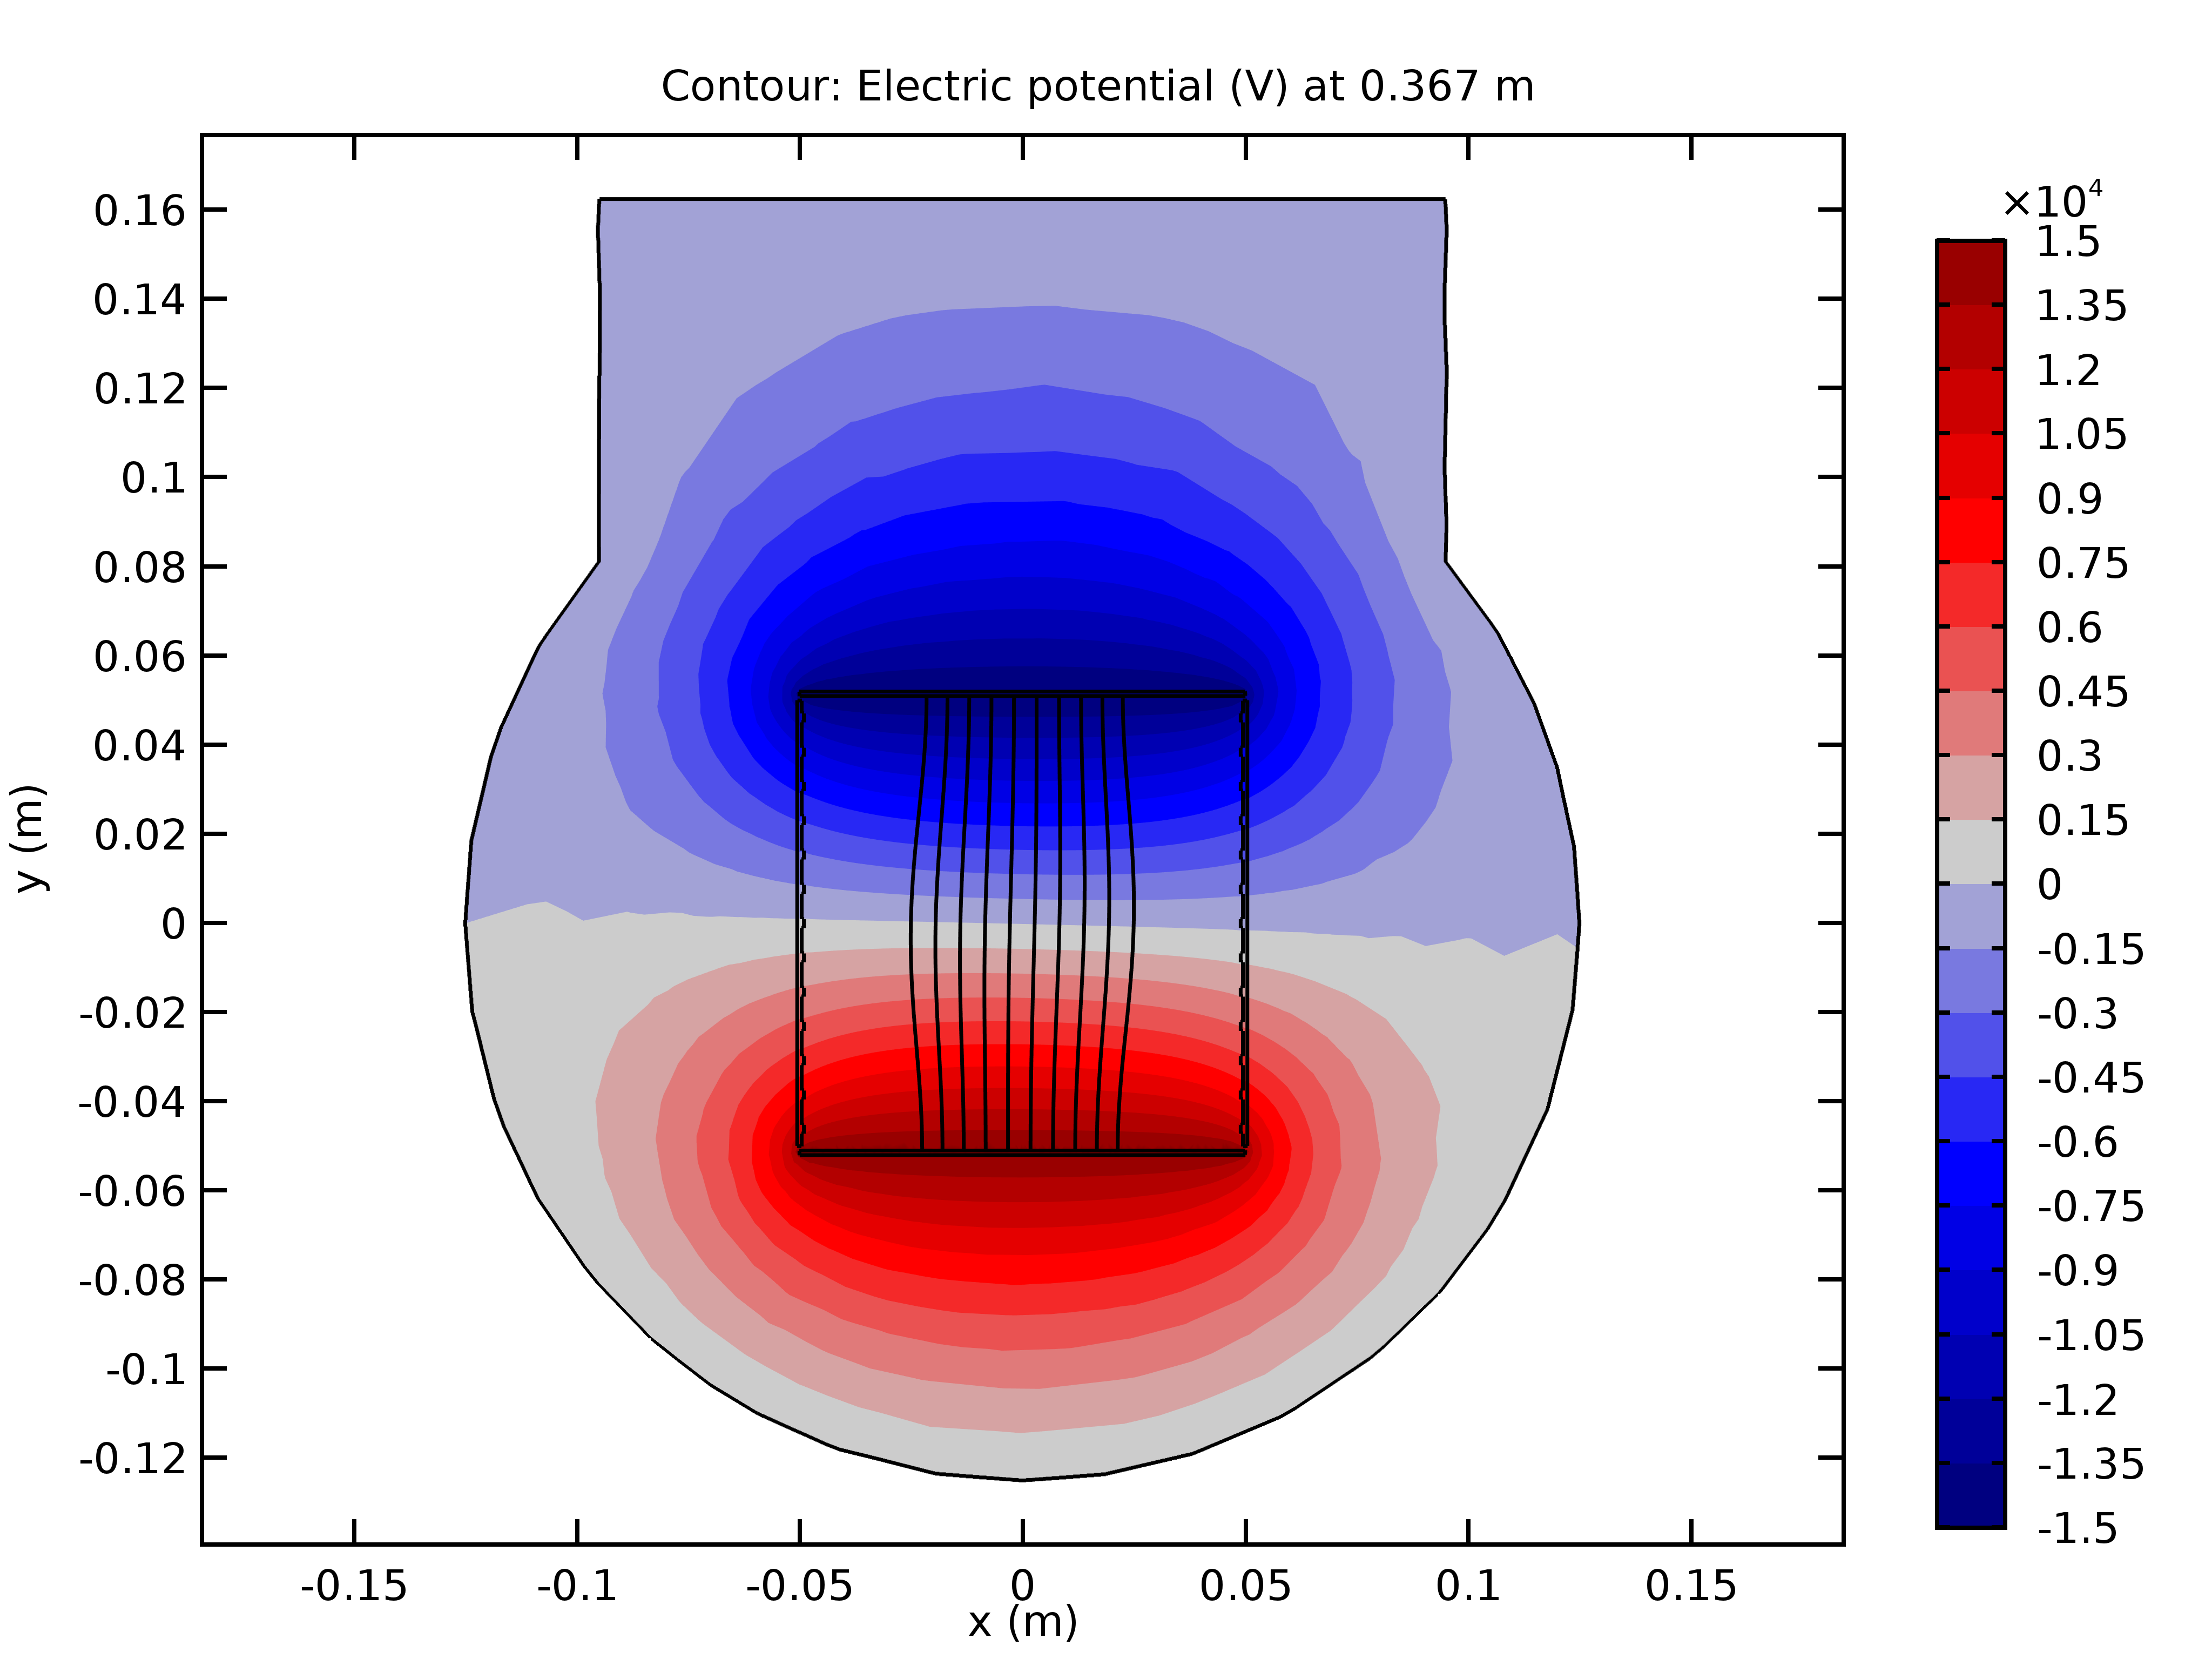
\includegraphics[width=\textwidth]{03_Prototype/figures/fig021_image_asym_sym_b.png}
		\caption{Symmetric configuration.}
		\label{chap3:asym_sym_b}
	\end{subfigure}
	~
	\begin{subfigure}{0.5\textwidth}
		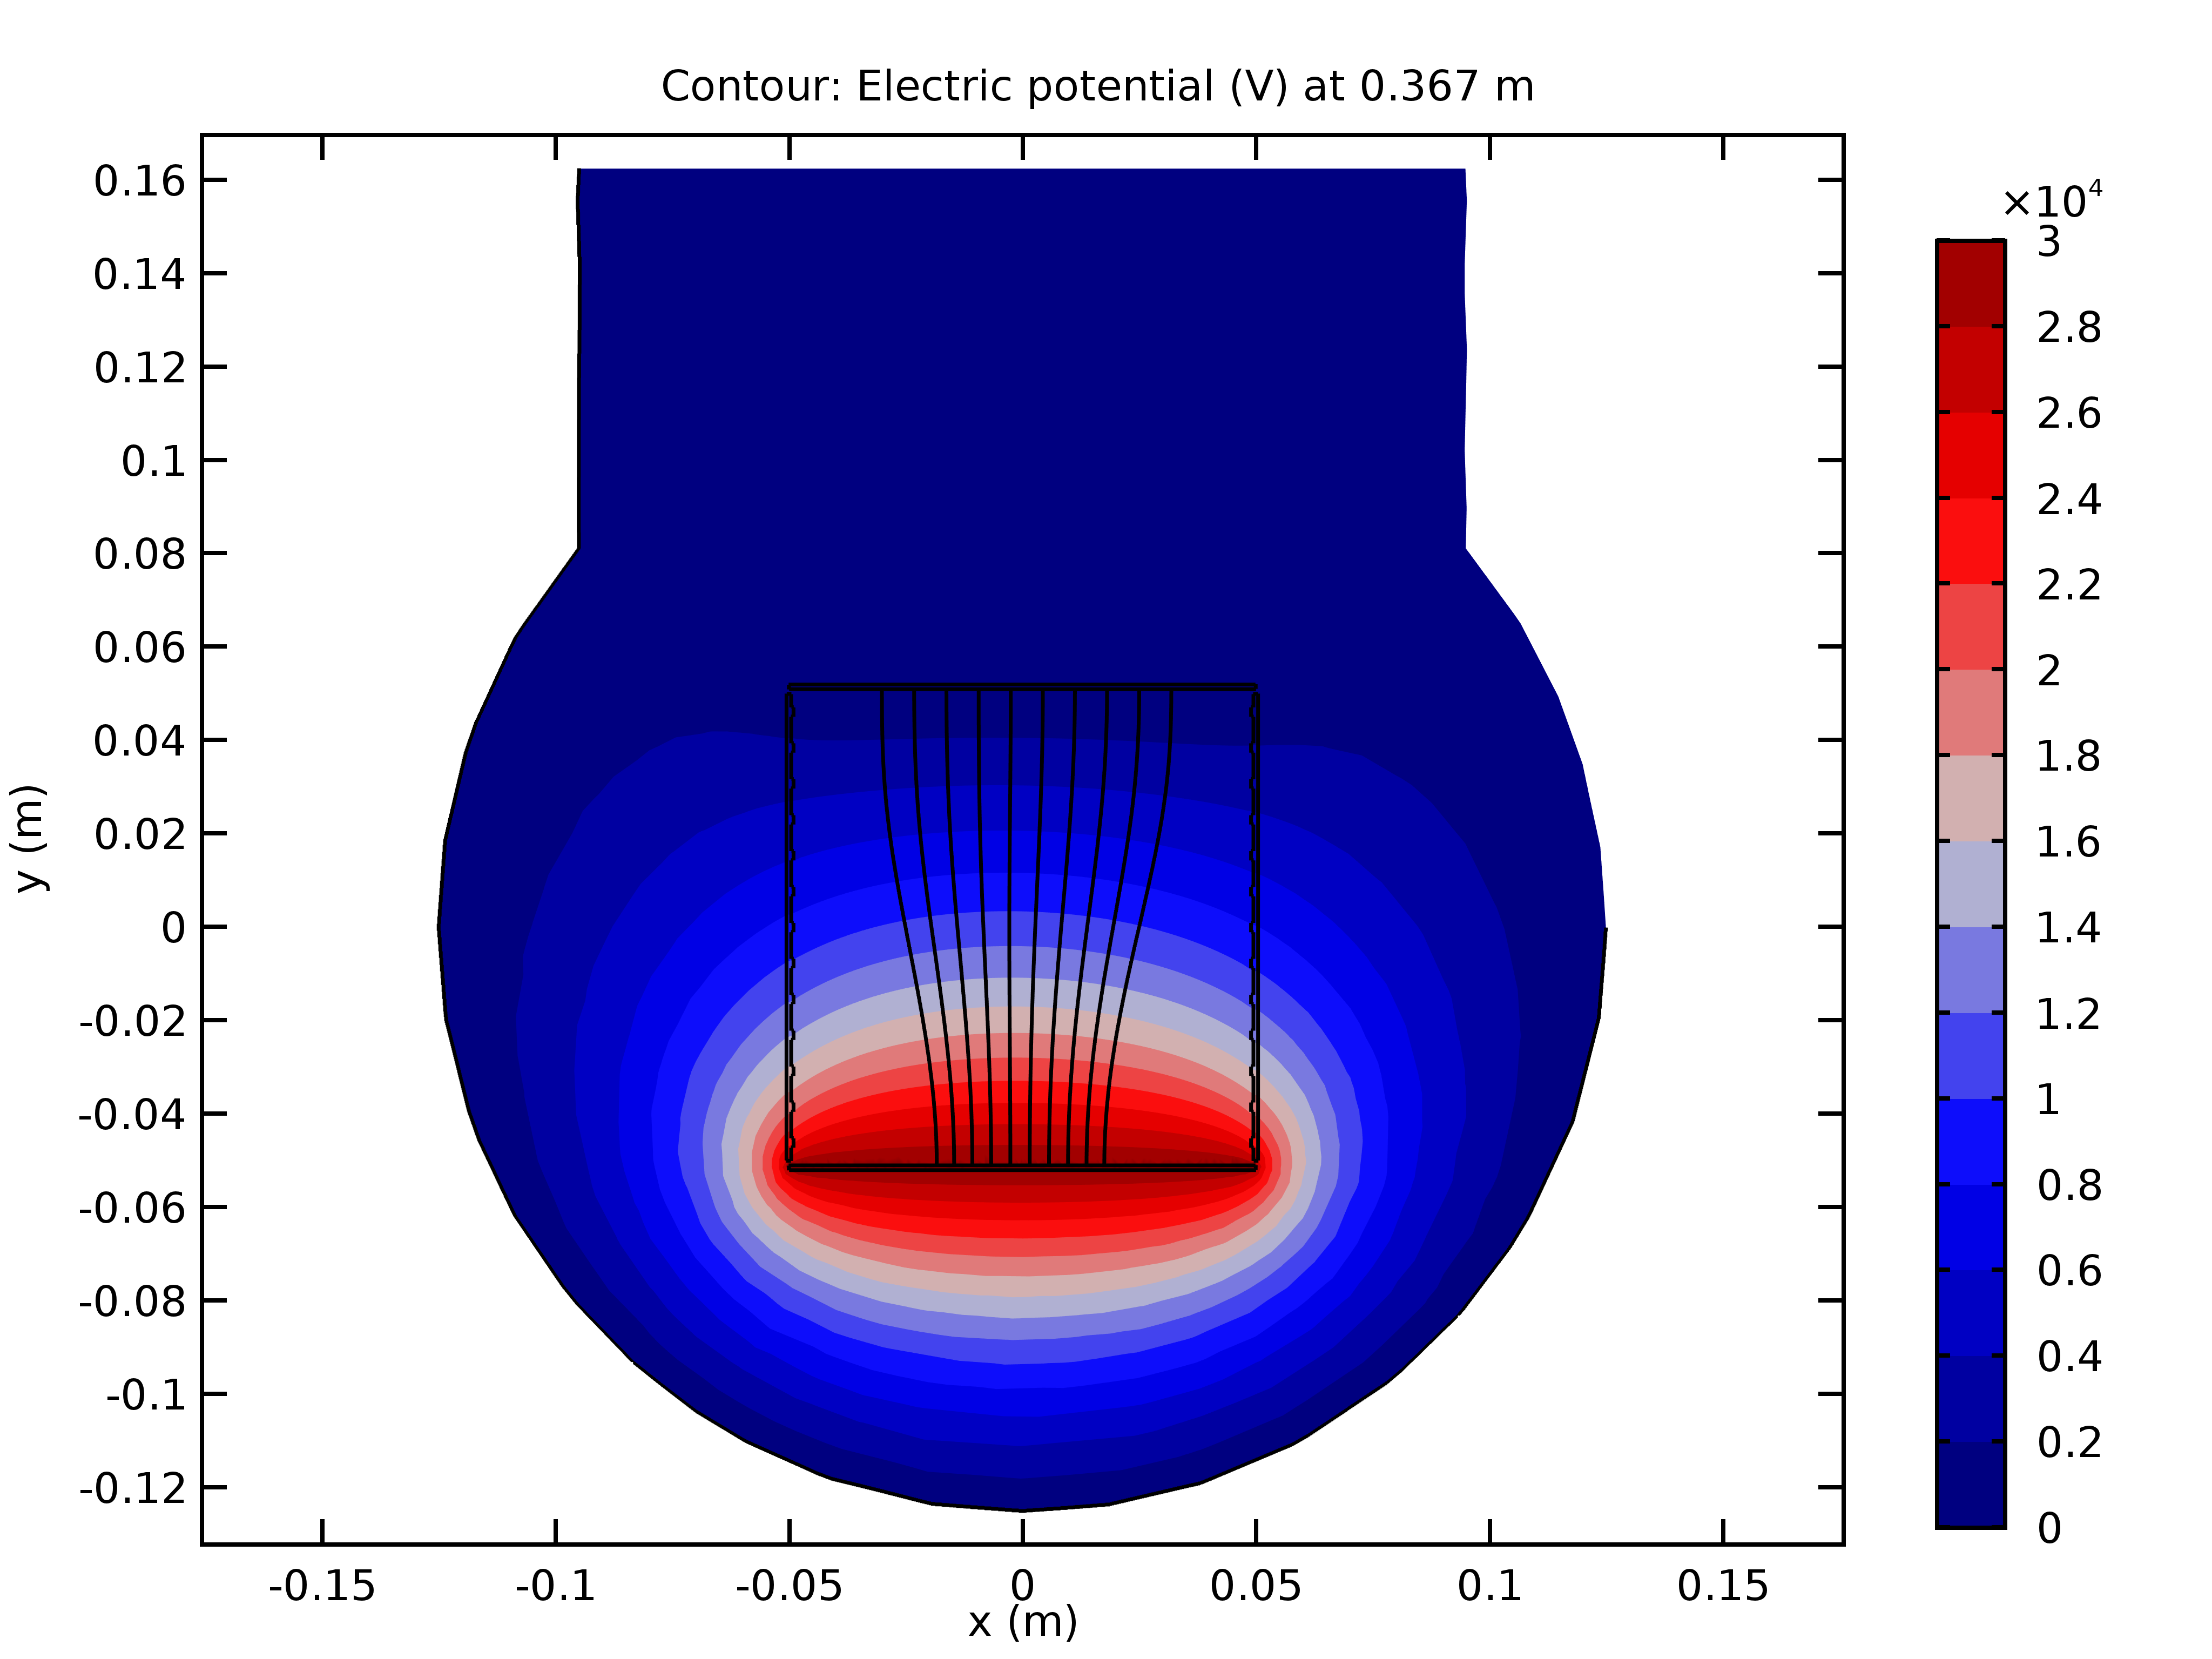
\includegraphics[width=\textwidth]{03_Prototype/figures/fig021_image_asym_sym_a.png}
		\caption{Asymmetric configuration.}
		\label{chap3:asym_sym_a}
	\end{subfigure}
	\caption[Comparison between symmetric and asymmetric configuration]{Comparison between symmetric and asymmetric configuration.}
	\label{chap3:asym_sym}
\end{figure}


  In this configuration (Fig. \ref{chap3:asym_sym_b}), the field focuses the particles in the transverse plane but also in the longitudinal plane. This explains why the particle number on the readout is higher than the expected number. For this configuration, only the transverse plane should be corrected.

  In asymmetric configuration (Fig. \ref{chap3:asym_sym_a}), the field is defocusing in the transverse plane, but also in the  longitudinal one. The projection of the beam will be much broader than expected and many particles are lost during the particle drifts. Therefore, the electric field must be improved in both planes.


  \subsection{IPM cross-interaction}

  The \acrshort{ipm}s are in close proximity due to the limited room of the vacuum chamber, in order to measure the beam profile in both  transverse  directions at the same location. This proximity leads to a coupling effect between the two \acrshort{ipm}s due to fringe fields. Moreover, the uniformity of the electric field is strongly related to the geometry that encloses the \acrshort{ipm}s. The \acrshort{lwu} walls are at ground potential, hence the uniformity of the electric field in the \acrshort{ipm}s depends on their position in the \acrshort{lwu}. This means that the electric field in each \acrshort{ipm} has to be corrected individually.

  We simulated in COMSOL different \acrshort{ipm} configurations with and without grounded disks separating the \acrshort{ipm}s and located at different positions. The \acrshort{ipm}s cannot be shifted too much in the inner volume of the vacuum vessel because the space is limited by the WS on the left and by the \acrshort{lwu} walls on the right. 
  
  Fig. \ref{chap3:IPM_disk} shows the quadratic mean values for each electrical field component (as described in section \ref{chap3:sec:criteria}) inside the geometry of the LWU with the two IPMs implemented. When disks are present, the fields $E_{x}$ and $E_{y}$ are constrained within the space in-between them. The cross interaction effect is not lowered, but more flattened. This means that the effect on profile is constant over the readout size. 
  Also with disks, the minimum $E_{z}$ value is in the middle of the IPMs, so the readout location is the same for the both IPMs.
  Note that the field shapes of IPM1 and IPM2 look more similar when disk are present, because electric field is less dependant to the \acrshort{lwu} geometry. This effect is quite useful because the same corrections can be applied to both \acrshort{ipm}s, simplifying the optimization of field correctors. Using disks is therefore a straightforward solution to shield IPMs and to simplify the design of the IPMs .
  %This effect is particularly visible on $E_{z}$
  %This means that the field correction must be done for each IPM individually.
  %When disks are present
  
  %So, we found out that using disks improve the electric field uniformity, as shown on Fig. \ref{chap3:IPM_disk} where disk influences are displayed.

  \begin{figure}[!ht]
	\centering
	\begin{subfigure}{0.7\textwidth}
		\includesvg[width=\textwidth]{03_Prototype/figures/fig022_2IPM_ASYM_NODISK_NODEG_a}
		\caption[]{Electrical field without disk.}
		\label{chap3:no_disk}
	\end{subfigure}

	\begin{subfigure}{0.7\textwidth}
		\centering
		\includesvg[width=\textwidth]{03_Prototype/figures/fig022_2IPM_ASYM_DISK_NODEG_c}
		\caption{Electrical field with disks.}
		\label{chap3:disks}
	\end{subfigure}
	\caption[Influence of shielding disks on the IPM electric field]{Influence of shielding disks on the IPM electric field along the LWU.}
	\label{chap3:IPM_disk}
\end{figure}

  \vspace{1cm}

  %The quadratic mean values are plotted for each electrical component on the longitudinal axis of the \acrshort{ipm}, as described in section \ref{}. An important field overlapping occurs when no disk is mounted between the two \acrshort{ipm}s. When disks are present, the fields are constrained within the space in-between them and the cross interaction effect is reduced. On the other hand, the field variations are sharper in this area, so the longitudinal field component is worse with disks. Note that the field shape is identical in both \acrshort{ipm}s since they are independent of the \acrshort{lwu} geometry. This is quite useful because the same corrections can be applied to both \acrshort{ipm}s and it simplifies the optimization of field correctors.

  \subsection{Field corrections}
  \label{chap3:field_corrections}
  \begin{wrapfigure}{r}{0.45\textwidth}
	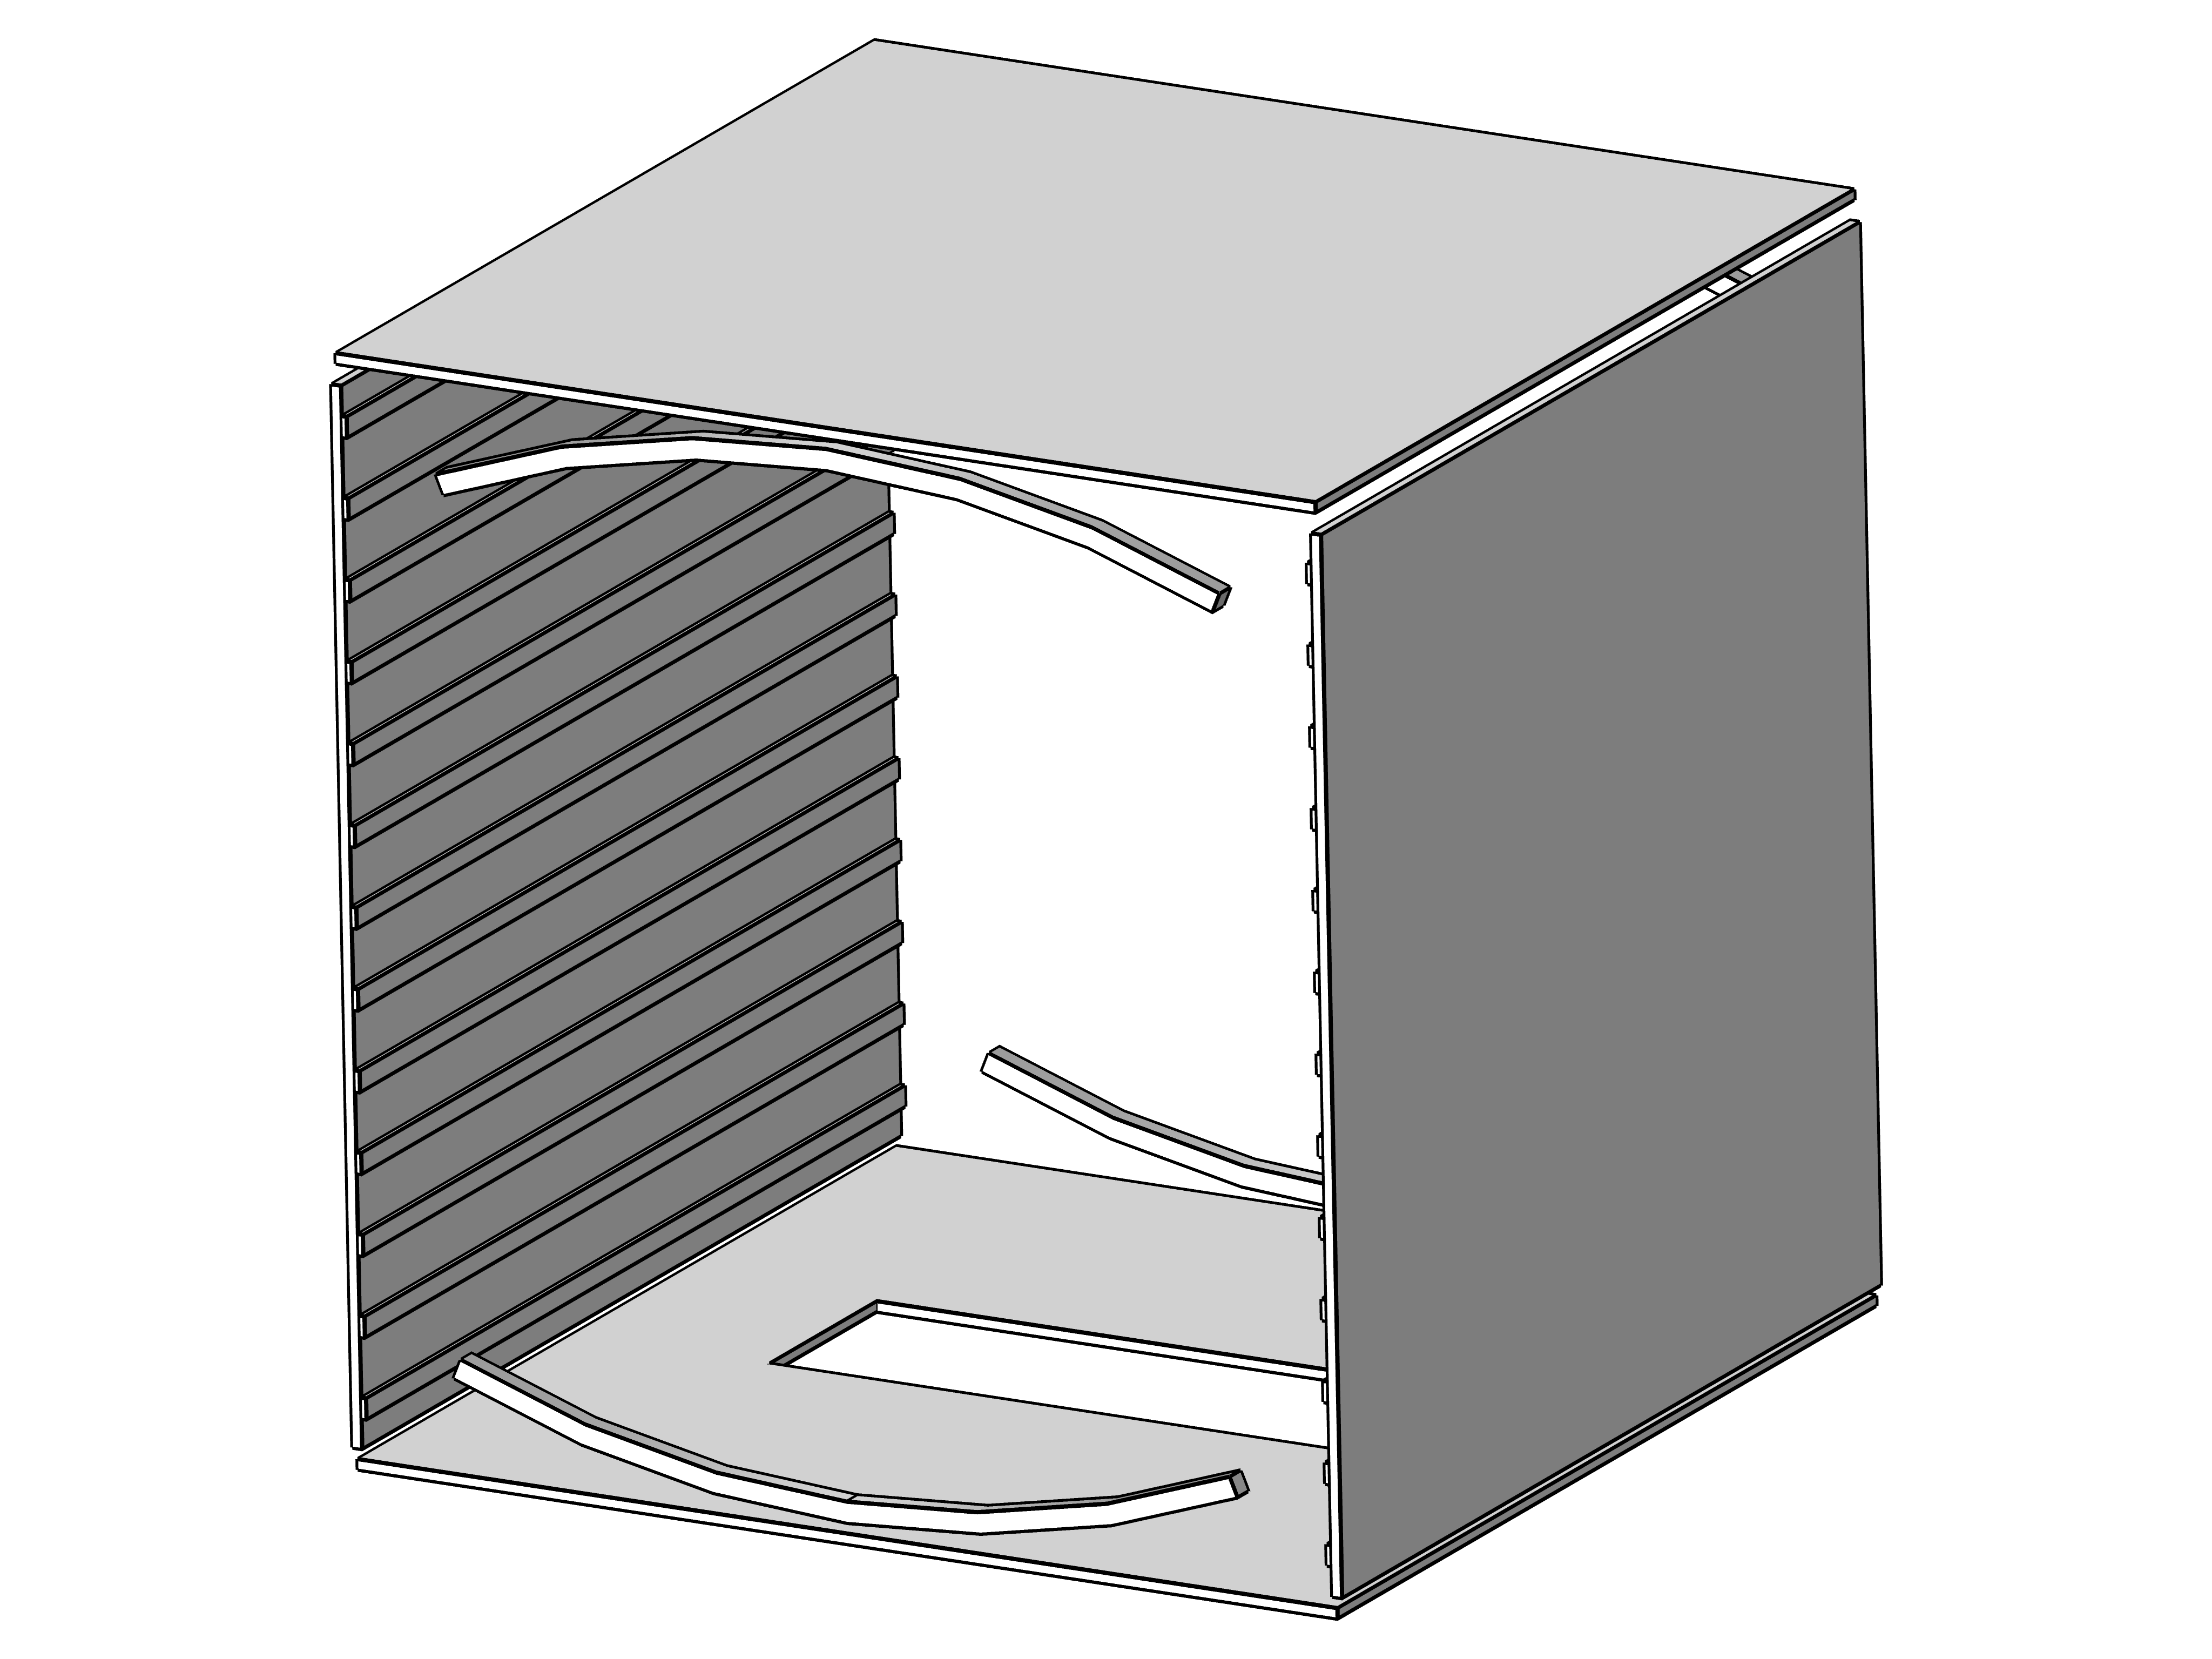
\includegraphics[width=0.45\textwidth]{03_Prototype/figures/fig026_IPM_COMSOL.png}
	\caption[IPM geometry in COMSOL]{IPM geometry in COMSOL.}
	\label{chap3:IPM_COMSOL}
\end{wrapfigure}

  The electric field is improved by means of field correctors (also called field degraders) and the curved electrode pairs. Fig. \ref{chap3:IPM_COMSOL} shows the COMSOL geometry of an example of \acrshort{ipm} that has been simulated. One can see the degraders on each side and the curved electrodes at the top and bottom of each \acrshort{ipm}.

  The field correctors will constrain the electric potential on the side of the \acrshort{ipm}. Thus, the iso-potential will be more flat in the \acrshort{ipm}, leading to a better electric field uniformity. In practice, field degraders are just conductive strips connected to a voltage
  source directly powered by HV. One can directly connect them to power supplies. This method would allow to finely tune the potential on the electrodes, but it would also require HV feedthroughs for each electric potential. Unfortunately, we could not implement this solution since the available space on the \acrshort{ipm} flange is restricted. We instead exploited directly the existing high voltages used for polarizing the \acrshort{ipm} electrodes for feeding a resistor bridge as shown in Fig. \ref{chap3:resistor_chain}. The potential at each field corrector is simply given by the Ohm law:
  \begin{equation}
    V_{i} = \frac{\sum_{k = 1}^{i} R_{k}}{\sum_{j = 1}^{N} R_{j}}V_{HV} \label{chap3:PontDiviseur}
  \end{equation}

  \begin{wrapfigure}{l}{0.3\textwidth}
	\begin{center}
		\begin{tikzpicture}[scale=0.8,transform shape,american voltages]
			\draw (0,0) node[label={above:HV}] {} to [short, *-] (2,0)
			to [R, l_=$R_1$] (2,2)
			to [R, l_=$R_2$, *-] (2,4);
			\draw (0, 9) node[label={above:HV}] {} to [short, *-] (2,9)
			to [R, l_=$R_{N}$] (2,7)
			to [R, l_=$R_{N-1}$, *-] (2,5)
			(2,4.5) node[] {...};
		\end{tikzpicture}
	\end{center}
	\caption[Resistor chain]{Resistor chain.}
	\label{chap3:resistor_chain}
\end{wrapfigure}


  This method has some drawbacks. The choice of resistors is limited, since not all resistance values are commercially available \cite{Vishay2012}. In addition, the use of resistors in a clean vacuum is not really recommended since it often requires welding. Also, the resistors should be able to sustain high radioactive levels, mainly considering that, if one of them is damaged the entire bridge is affected.

  Finally we decided to use $13$ degraders, regularly spaced by $7.5\,\mathrm{mm}$ from each other, on each side of the \acrshort{ipm}. A degrader is $2\,\mathrm{mm}$ width and $100\,\mathrm{mm}$ long (in longitudinal direction). The $7^{th}$ degrader is located in the middle plane of the \acrshort{ipm}.

  The electric potential value which gives the best uniformity is computed with COMSOL for each degrader. The resistor chain is determined from these values with respect to the equation (\ref{chap3:PontDiviseur}). For each corrector, two commercial resistors are mounted in series allowing values as close as possible to the optimal one. Resistors are selected within the $\mathrm{M}\Omega $ range, reducing the power consumption of power supplies. The field simulation is recomputed with the real resistors and potential values.

  In the case of the symmetrical \acrshort{ipm}, only the first $6$ degraders must be calculated since the $7^{th}$ is grounded and the last $6$ potentials are held at opposite potentials with respect to  the first 6 ones. The voltage and resistor values of the degrader chain for symmetric \acrshort{ipm} are tabulated in the Table \ref{chap3:resistor_sym}.

  \begin{table}[ht]
	\centering
	\caption[Description of the resistor chain for the field degraders in the symmetric IPM]
	{Description of the resistor chain for the field degraders in the symmetric IPM.}
	\label{chap3:resistor_sym}
	\begin{tabular}{lllllllll}
		\toprule
		                                & 1  & 2     & 3      & 4    & 5      & 6     & 7    &    \\
		\midrule
		%Voltage (\(\mathrm{kV}\))       & 15 & 13.57 & 11.32  & 8.72  & 6.52   & 4.31  & 2.16 & 0  \\
		%Resistor (\(\mathrm{M}\Omega\)) &    & 13.24 & 20.83  & 24.07 & 20.37  & 20.46 & 19.9 & 20 \\
		Resistor (\(\mathrm{M}\Omega\)) &    & 13.4  & 20.715 & 24.3 & 20.332 & 20.51 & 20   & 20 \\
		Voltage (\(\mathrm{kV}\))       & 15 & 13.56 & 11.32  & 8.71 & 6.52   & 4.31  & 2.15 & 0  \\
		\bottomrule
	\end{tabular}
\end{table}
  \begin{figure}[!h]
	\begin{center}
		\includesvg[width=\textwidth]{03_Prototype/figures/fig023_SymTransversalProfile}
	\end{center}
	\caption[Particle tracking for real symmetric field configuration with and without configuration]{Particle tracking for real symmetric field configuration with and without configuration (degraders and disks). Beam is assumed to be gaussian with a size $\sigma_{beam}=3\,\mathrm{mm}$ [Image à refaire]}
	\label{chap3:SymTransversalProfile}
\end{figure}


  A particle tracking was performed with the real corrected field and the results are shown in Fig. \ref{chap3:SymTransversalProfile}. Note that, even without correction, the symmetrical \acrshort{ipm} gives fairly good results. The focusing effect, shown in the previous section, is visible and explains why there are more particles on readout than expected. When the field correctors are enabled, the profile is extremely well reconstructed with an error of less than $0.2\,\mathrm{\%}$.  This fulfills the requirements of \acrshort{ess} on the profile error.

  
  For the asymmetric \acrshort{ipm}, we proceeded in the same way. Also in this case, the resistor chain had to be optimized as well as the two curved electrodes. Table \ref{chap3:resistor_asym} gives the values of resistances and potentials in the case of the asymmetric \acrshort{ipm}.

  \begin{table}[ht]
  \noindent
  \caption[Description of the resistor chain for the field degraders and curved electrodes in the asymmetric IPM]
  {Description of the resistor chain for the field degraders and curved electrodes in the asymmetric IPM. [A finir je dois remplir avec les bonnes valeurs]}
  \label{chap3:resistor_asym}
  \begin{tabular}{llllllllll}
    \toprule
                                    & Curved &      & HT    &      & 1     &      & 2    &      & 3    \\
    \midrule
    Resistor (\(\mathrm{M}\Omega\)) &        & 20.5 &       & 17.2 &       & 15.5 &      & 22.2        \\
    Voltage (\(\mathrm{kV}\))       & 30     &      & 27.63 &      & 25.64 &      & 23.85 &      & 21.29 \\
    \bottomrule
  \end{tabular}
  \\
  \medskip
  \begin{tabular}{lllllllllll}
    \toprule
                           &      & 4  &      & 5  &    & 6  &      & 7  &      & 8  \\
    \midrule
    Resistor (\(\mathrm{M}\Omega\)) & 24.1 &    & 19.5 &    & 20 &    & 19.5 &    & 13.5      \\
    Voltage (\(\mathrm{kV}\))       &      & 18.5 &      & 16.25 &    & 13.94 &      & 11.69 &      & 10.13 \\
    \bottomrule
  \end{tabular}
  \\
  \medskip
  \begin{tabular}{lllllllllll}
    \toprule
                           &    & 9  &      & 10 &      & 11 &       & 12 &      & 13 \\
    \midrule
    Resistor (\(\mathrm{M}\Omega\)) & 16 &    & 17.2 &    & 13.4 &    & 18.51 &    & 13.5      \\
    Voltage (\(\mathrm{kV}\))       &    & 8.28 &      & 6.3 &      & 4.74 &       & 2.6 &      & 1.05 \\
    \bottomrule
  \end{tabular}
  \\
  \medskip
  \begin{tabular}{llll}
    \toprule
                           &     & Gnd & Curved \\
    \midrule
    Resistor (\(\mathrm{M}\Omega\)) & 9.1 &     &        \\
    Voltage (\(\mathrm{kV}\))       &     & 0  & 2850      \\
    \bottomrule
  \end{tabular}

\end{table}
  \begin{figure}[!h]
	\begin{center}
		\includesvg[width=\textwidth]{03_Prototype/figures/fig025_AsymTransversalProfile}
	\end{center}
	\caption[Particle tracking for real asymmetric field configuration with and without configuration]{Particle tracking for real asymmetric field configuration with and without configuration (degraders and disks). Beam is assumed to be gaussian with a size $\sigma_{beam}=3\,\mathrm{mm}$.}
	\label{chap3:AsymTransversalProfile}
\end{figure}


  The results of the particle tracking for this case, are shown in Fig. \ref{chap3:AsymTransversalProfile}. The asymmetric field defocuses particles in both directions when the correctors are missing. So the reconstructed profile is $35\,\mathrm{\%}$ wider and some particles do not even reach the readout. The shift in position is due to the cross interaction between the two \acrshort{ipm}s. When corrections are enabled, the obtained transverse profile is much better: the error on the profile is only $0.4\,\mathrm{\%}$. The position is also corrected thanks to the shielding disks and curved electrodes, therefore no more shift appears. However, the correction on the longitudinal field is not as good as in the case of symmetric configuration and some particles are still lost during the drift: only $77\,\mathrm{\%}$ of the particles will reach the readout.


  \subsection{Grid}
  \label{chap3:sec:grid}
  As shown in Fig. \ref{chap3:IPM_COMSOL}, the readout electrode is not completely filled: a rectangular slit allows the ions or electrons to move toward the readout system. This slit is relatively big ($2\times5\,\mathrm{cm^{2}}$) with respect to the electrode dimensions ($10\times10\,\mathrm{cm^{2}}$), so it affects the electric field uniformity. A wire mesh can easily overcome this problem. Indeed in the close proximity of the mesh the field is not very straight, but at farther distances the field becomes constant. The mesh allows to have always the same field uniformity in the \acrshort{ipm} whatever readout is used. On the other hand, it represents an obstacle for the incident particles, therefore the grid must be chosen carefully.

  Actually, many of our colleagues are involved in the development of Micromegas detectors \cite{GIOMATARIS199629}. So we have access to several types of mesh. We started with a stainless steel mesh with a pitch of $450\,\mathrm{\mu m}$ and a wire size of $50\,\mathrm{\mu m}$, so the optical transparency is about $90\,\mathrm{\%}$. A first approximation can be made with the Fourier series of the electric potential as proposed by Feynman \cite{feynman2011feynman}:
  \begin{equation}
    V(x,y)= \sum^{\infty}_{n=0} A_{n} \cdot cos(-\frac{2\pi n x}{\lambda}) \cdot exp(-\frac{2\pi n y}{\lambda})
  \end{equation}

  In this case the grid is regularly spaced in the $x$ direction by a step $\lambda$. If we are at a distance $k \cdot \lambda$ away from the grid the first harmonic is attenuated by a factor $e^{-2\pi k}$. This tendency can be easily confirmed with the FEM or BEM method. Fig. \ref{chap3:Grid} shows the electrical potential close to the mesh for two different field configurations. One can see that the field is almost constant starting from less than $1\,\mathrm{mm}$ distance from the mesh. So there will be no problem using this grid.

  \begin{figure}[!ht]
	\centering
	\begin{subfigure}{\textwidth}
		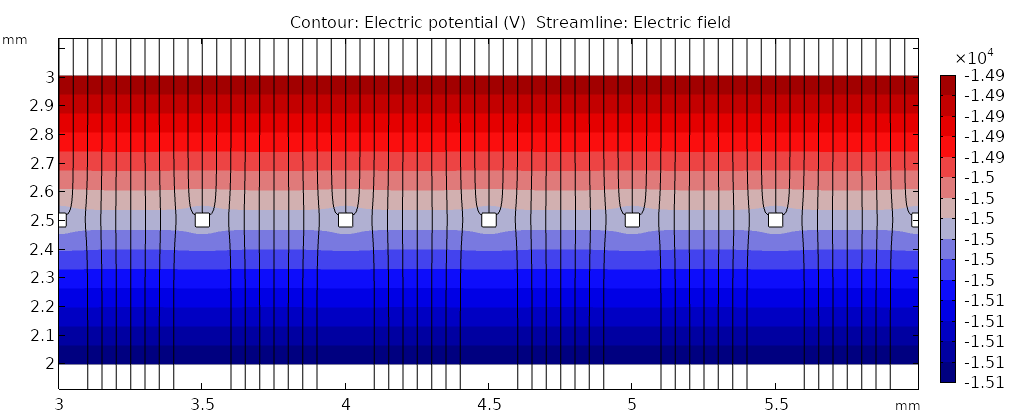
\includegraphics[width=\textwidth]{03_Prototype/figures/fig027_Grid1.png}
		\caption[]{Configuration 1: The field is constant (up: \(3\,\mathrm{kV/cm}\); down: \(3\,\mathrm{kV/cm}\)). The mesh transmission is close to the optical transparency.}
		\label{chap3:Grid1}
	\end{subfigure}

	\begin{subfigure}{\textwidth}
		\centering
		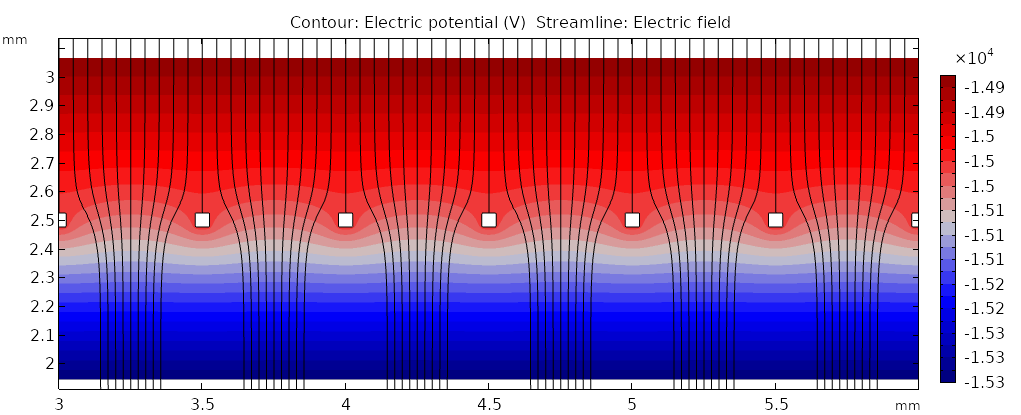
\includegraphics[width=\textwidth]{03_Prototype/figures/fig027_Grid2.png}
		\caption[]{Configuration 1: The field is higher below the grid (up: \(3\,\mathrm{kV/cm}\); down: \(6\,\mathrm{kV/cm}\)). The mesh transmission is higher than the optical transparency.}
		\label{chap3:Grid2}
	\end{subfigure}
	\caption[Electrical simulations of a \(50/450\,\mathrm{\mu m}\) grid]{Electrical simulations of a \(50/450\,\mathrm{\mu m}\) grid. Two different field configurations were simulated. Both shows that the electrical field becomes uniform few mm away from grid. However the particle transmission differs due different ratios of the electric fields imposed in the two regions.}
	\label{chap3:Grid}
\end{figure}


  The grid is an obstacle for the incoming particles, and the number of stopped particles is directly related to the optical transparency of the grid. However it is possible to improve the transmission by increasing the field on one side of the grid. A simple analytical model has been demonstrated in the case of wire grid \cite{Bunemann1949}. We assume that our grid follows this model\footnote{This is not really true since our grid is not made of cylindric wires.}:
  \begin{equation}
    \frac{E_{r}}{E_{d}} \geq \frac{1+\frac{2 \pi r}{\lambda}}{1-\frac{2 \pi r}{\lambda}}
  \end{equation}
  where $E_{r}$ is the field on the readout region, $E_{d}$ is the field on the drift region and $r$ the wire diameter. For our grid configuration the ratio $\frac{E_{r}}{E_{d}}$ must be higher than $4.38$.
  An example is given in Fig. \ref{chap3:Grid}. The top figure shows a case where $E_{r}=E_{d}$. The field lines may be stopped by the grid wires. In the bottom figure, $E_{r}=2 \cdot E_{d}$ and the field lines are attracted into the readout region due to the field difference.

  The grid can be polarized in order to use it as a Frish grid. For some readout, it allows to get rid of certain signal contributions. More details will be given in section \ref{chap3:ramo} of this chapter.

  Finally, the grid may be also used to shield the readouts against possible electromagnetic noises created by all the radio-frequency devices. The effectiveness of the grid is clear. The wavelengths for the two \acrshort{ess} frequencies\footnote{We only considered the first harmonic.} are respectively $80\,\mathrm{cm}$ and $40\,\mathrm{cm}$. The pitch of our grid is far less than theses wavelengths.

  %\subsection{Summary}

  \section{Initial momentum}
  So far, we assumed that the ions and/or electrons were created without initial velocity i.e. at rest in a pure electric field. In this case, electrons and ions give same results and the value of the extraction field does not matter. In reality, these particles have a non-negligible initial speed and may be affected by parasitic electromagnetic fields. This can greatly affect the profile, thus the extraction field must be increased in order to minimize such distortion. In the following sections, we will try quantify these effects to determine the nominal value of the extraction field.
  %The second limitation concerns possible \acrshort{hv} breakdowns. In very high vacuum a distance of some millimeter is sufficient to isolate several tens of kilovolts. However, the breakdowns are also strongly influenced by the surface states of the electrodes, the composition of the vacuum and the presence of leakage current \cite{Latham1995}. Hence, we should keep a standoff distance between the electrode and the vacuum vessel (less than 1kV/cm between the \acrshort{ipm}s and \acrshort{lwu}).

  \subsection{Thermal distribution}
  A first approximation of the initial speed of ions can be done thanks to the distribution of Maxwell-Boltzmann. The distribution of the speeds with respect to the particle mass and the temperature is given by the following equation:

  \begin{equation}
    F(\boldsymbol{v}) = \left(\frac{m_{part}}{2 \pi k_{b} T}\right)^{\frac{3}{2}}\exp\left(-\frac{m_{part}\boldsymbol{v}^{2}}{2 k_{b} T}\right)
  \end{equation}
  % \begin{wrapfigure}{r}{0.5\textwidth}
% 	\includesvg[width=0.5\textwidth]{03_Prototype/figures/fig013_maxwell_gas2}
% 	\caption[Maxwell-Boltzmann distribution for some species of ESS residual gas]{Maxwell-Boltzmann distribution for some species of ESS residual gas.}
% 	\label{chap3:maxwell_gas}
% \end{wrapfigure}
\begin{figure}[!ht]
	\centering
	\includesvg[width=0.7\textwidth]{03_Prototype/figures/fig013_maxwell_gas2}
	\caption[Maxwell-Boltzmann distribution for some species of ESS residual gas]{Maxwell-Boltzmann distribution for some species of ESS residual gas.}
	\label{chap3:maxwell_gas}
\end{figure}
  Where, $k_{b}$ is the Boltzmann constant, $T$ the temperature, $\boldsymbol{v}$ is the speed vector of the considered particle and $m_{part}$ its mass. The Maxwell-Boltzmann distribution works well for perfect gases at low densities. We assumed that is true for the \acrshort{ess} residual gas. The speed is uniformly distributed along all directions ($4\pi$).

  The Fig. \ref{chap3:maxwell_gas} shows the normalized distributions for some of the molecules present in the \acrshort{ess} residual gas. One can see directly that the speed of the fastest ion is below $5000\,\mathrm{m/s}$. A field of few hundred volts per centimeter is more than enough to compensate this effect. It gives no significant difference during the particle tracking. So, we can completely neglect the thermal motion for ions.

  \subsection{Momentum transfer during ionization process}
  Garfield++ can be used again to quantify the spectra of the momentum and the energy transfered to the ionized electrons. Fig. \ref{chap3:garfieldangle} shows this energy spectrum and the emission angle (or polar angle) distribution for several energies of a proton beam ($\sigma$ = 3 mm). The energy follows a Landau-like distribution with some Auger electrons. The polar angle is calculated with respect to the direction of the beam, while the azimuthal angle is uniform with respect to the transverse plane. A large proportion of electrons are perpendicularly ejected to the direction of propagation.

  \begin{figure}[!ht]
	\begin{subfigure}{0.5\textwidth}
		\includesvg[width=\textwidth]{03_Prototype/figures/fig028_garfield_energy.svg}
		\caption{Electron energy distribution.}
		\label{}
	\end{subfigure}
	~
	\begin{subfigure}{0.5\textwidth}
		\includesvg[width=\textwidth]{03_Prototype/figures/fig028_garfieldangle_2.svg}
		\caption{Electron emission angle distribution}
		\label{}
	\end{subfigure}
	\caption[Energy and emission angle of the ionized electrons]{Energy and emission angle of the ionized electrons.}
	\label{chap3:garfieldangle}
\end{figure}


  Particle tracking can be performed in order to quantify the influence of the initial momentum of electrons. Fig. \ref{chap3:ElectronProfile_a} presents the relative error on the profile caused by the initial energy as a function of the extraction field. Note that it is impossible to fully compensate the error with realistic electric field values (below $6\,\mathrm{kV/cm}$). Usually, when a profiler works in electron mode, a magnetic field parallel to the extraction field is added forcing the electrons to spin around the field direction. In the Fig. \ref{chap3:ElectronProfile_b}, a general example of correction done with a magnetic field is presented. In the range of $10^{-3}$ to $5\cdot10^{-2}\,\mathrm{T}$, the Larmor radius is still too high to constraint electrons drifting along the field lines.
  %and electrons does not have the time to spin several time during their drift. 
  A magnetic field of at least $0.1\,\mathrm{T}$ completely compensates the initial momentum of electrons. However the generation of such a magnetic field requires imposing dipole magnets. At \acrshort{ess} this solution is not feasible because the available space on \acrshort{lwu} is not sufficient to put two magnets close-by.

  \begin{figure}[!ht]
	\begin{subfigure}[t]{0.5\textwidth}
		\includesvg[width=\textwidth]{03_Prototype/figures/fig032_ElectronProfile_a.svg}
		\caption{Relative error on $\sigma_{beam}$ for different extraction fields.}
		\label{chap3:ElectronProfile_a}
	\end{subfigure}
	~
	\begin{subfigure}[t]{0.5\textwidth}
		\includesvg[width=\textwidth]{03_Prototype/figures/fig032_ElectronProfile_b.svg}
		\caption{Relative error on $\sigma_{beam}$ at constant extraction field of $1\,\mathrm{kV/cm}$ for various magnetic fields.}
		\label{chap3:ElectronProfile_b}
	\end{subfigure}
	\caption[Results from particle tracking with electrons considering initial energy]{Results from particle tracking with electrons considering initial energy.}
	\label{chap3:ElectronProfile}
\end{figure}

  We wanted to study the ion behavior, but unfortunately Garfield++ does not give the energy spectrum of the ions.
  %% Thus, we have considered two approaches for determining the ion energy. First, one assumes that the ions have the same energy as electrons and particle tracking gives same as electrons without magnetic field and the profile can not be corrected with realistic magnetic field value.&&
  We have considered the momentum conservation of a pure ionization process, meaning the molecule dissociation in one electron and an ion. The ion momenta follow then the same electron distribution depicted by Garfield++. Therefore, the speed of a ion is proportional to the speed of electron weighted by their mass ratio. For instance, the speed of a $100\,\mathrm{eV}$ electron is around $5.9\cdot10^{6}\,\mathrm{m/s}$, while the $H_{2}^{+}$ ion speed is only $1614\,\mathrm{m/s}$. In these conditions, the speed of ions is below the thermal motion and calculations are therefore useless.


  \section{Space charge effect}
  The last effect that can greatly affect the measurement of the profile is the Space Charge. The protons of the beam bunches are in motion, so a strong radial electric field and a circular magnetic field are created around the beam axis. Each \acrshort{ess} bunch is composed of $10^{9}$ protons. The effect of the space charge is not intuitive: electrons are light and may see less bunches but they are more sensitive to magnetic field. On the other hand, the ions are more massive and less sensitive to the EM fields but will undergo these fields many more times. Therefore, simulations were carried out to quantify this effect.

  The space charge effect is a critical aspect of IPMs in general and several simulations were developed or are under development \cite{Sapinski2016,IPMcolab2019}. Recently, a python framework dedicated to the IPM simulations, including space charge effects, has been released \cite{Vilsmeier2019}. The code is developed at GSI but is open to everyone. However in this thesis, only the in-house code developed by ESS and CEA will be described.

  \subsection{Lorentz transformation of electromagnetic fields}
  The physic basis behind the space charge remains the Maxwell equations presented in the section \ref{chap3:sec:maxwell}. These equations were unified before the discovery of special relativity by Einstein in 1905 but it appears that they were already compatible with special relativity \cite{feynman2011feynman}.

  Let's consider a simple case. A frame $F\prime$ is in motion with the speed $v$ along the $z$ axis with respect to frame $F$. The passage from one frame to the other is done by Lorentz transformation:
  \begin{align}
    \label{chap3:eqn:lorentz}
    \begin{split}
      ct\prime &= \gamma (ct - \beta z) ,
      \\
      x\prime &= x
      \\
      y\prime &= y
      \\
      z\prime &= \gamma (z - \beta ct)
    \end{split}
  \end{align}
  with $\beta$ and $\gamma$ the Lorentz factors.
  \begin{equation}
    \beta = \frac{v}{c}
    ,\
    \gamma = \frac{1}{\sqrt{1 - \beta^{2}}}
    %\label{eq5}
  \end{equation}
  The transformation is reverted by changing the sign of the lorentz factors in Eq (\ref{chap3:eqn:lorentz}).

  Now let's take charges moving in a same way. The charges are not subject to any acceleration and do not diverge \footnote{Without these two conditions, the Lorentz transformation must be computed with the tensor formalism \cite{feynman2011feynman}.}. In the frame $F$ the charges are in motion with $v$ speed while in the $F\prime$ the charges are completely immobile. Therefore in this frame the charges generate a purely electrostatic field, which can be computed using the Gauss's law.
  Electric and magnetic fields can be transformed as well:
  \begin{equation}
    \label{chap3:eqn:Elorentz}
    \boldsymbol{E} =
    \begin{pmatrix}
      \gamma \bar{E}_{x} \\
      \gamma \bar{E}_{y} \\
      \bar{E}_{z}
    \end{pmatrix}
    ,\
    \boldsymbol{B} =
    \begin{pmatrix}
      -\gamma v_{b} \frac{\bar{E}_y}{c^{2}} \\
      \gamma v_{b} \frac{\bar{E}_x}{c^{2}}  \\
      0
    \end{pmatrix}
  \end{equation}
  As a consequence, a purely electrostatic field in frame $F\prime$ gives an electromagnetic field in the frame $F$. This simple case outlines the space charge problematic: in an IPM the ionization by-products are affected by the electromagnetic field created by the pulse beam.


  \subsection{ESS/CEA Space Charge algorithm}
  A simulation code has been developed in the frame of a Collaboration between ESS and CEA, in order to quantify the effects of space charge on the profile measurement with respect to the \acrshort{ess} beam conditions \cite{Thomas-2016-1,Belloni2018}. The code is based on the analytical evaluation of the electric field for a Gaussian charge distribution and a full description of this model is available here \cite[Eq. (16-18)]{Wanzenberg2010}.

  A simplified workflow of the simulation program is given in the following section.
  A particle, ion or electron, is drawn according to the characteristics of the ESS beam, which is assumed to follow a gaussian distribution in 3D. The electric field of the beam is calculated in the moving frame from the equations given in the references. In this frame the beam width is spread by a factor. The resulting electromagnetic field in the frame of the IPM is calculated using the Lorentz transformations of fields. A Runge Kutta integrator computes the new particle position according to the electromagnetic field of the bunches and the extraction field of the IPM. At each integration step the fields of the beam are recalculated taking into account the new position of the bunches and the periodicity of the bunches. The particle is tracked until it reaches the readout plane.

  \subsection{Results}
  The effect of space charge depends on many beam parameters, therefore several simulations has been done to cover a wide range of ESS conditions. In the following only a small amount of the results is presented. %A detailed review of the results is available ...
  \begin{figure}[!ht]
	\begin{subfigure}[t]{0.5\textwidth}
		\includegraphics[width=\textwidth]{example-image-a}
		\caption{Error on the profile measurement, for electrons and $H_{2}^{+}$ ions, due to space charge effects versus the extraction field. The beam is assumed to be a Gaussian with $\sigma_{x}=\sigma_{x}=\sigma_{x}=2\,\mathrm{mm}$}
		\label{}
	\end{subfigure}
	~
	\begin{subfigure}[t]{0.5\textwidth}
		\includesvg[width=\textwidth]{03_Prototype/figures/fig000_SC_ions_electrons}
		\caption{Error on the profile measurement, for electrons and $H_{2}^{+}$ ions, due to space charge effects versus the extraction field. The beam is assumed to be a Gaussian with $\sigma_{x}=\sigma_{x}=\sigma_{x}=2\,\mathrm{mm}$}
		\label{}
	\end{subfigure}
	\caption[]{}
	\label{chap:}
\end{figure}


  Two interesting results are given in Fig. \ref{chap3:fig:SC}. On the left hand side, the relation between the space charge and the beam energy is shown. The space charge has a higher impact on the profile when protons are at lower energy. On the right hand side, the influence of the beam current on the measurement error is visible. As expected the error increases linearly with the beam current.


  In Fig. \ref{chap3:fig:SC_profile}, an example of the \acrshort{ess} beam size measured from profiles obtained with ions and electron is presented. The proton energy and beam current have been set to $90\,\mathrm{MeV}$ and $62.5\,\mathrm{mA}$. The value of the extraction field used in the simulation is chosen to be technically achievable. It is clear that the effect is stronger for electrons than for ions.

  %  The expected uncertainty for the beam size measurement is $10\,\mathrm{\%}$. The presented case shows the impact of the space charge can be strong, but yet the retrieved values are still within the requirements for the measurement uncertainty. Larger beam sizes are associated with weaker space charge effect, hence, the designed instrument is expected to deliver reliable information on the \acrshort{ess} beam profile and size.

  The duty cycle of the beam plays a role in the distortion of the profiles. Electrons, being light, reach the detector within the passage of one bunch, therefore they feel the combined electric and magnetic forces most of the time along their pass. On the other hand, ions are more massive and experience the passage of several bunches before reaching the detector.
  Hence, the forces from the bunches ions feel are weighted by the duty cycle of the varying electric field generated in $F\prime$. For the case of \acrshort{ess}, the bunches are $3\,\mathrm{ps}$ long, and the period between them is $2.84\,\mathrm{ns}$. So the integrated force seen by the ions is weaker than as the one experienced by the electrons.

  \begin{figure}[!ht]
	\begin{subfigure}[t]{0.5\textwidth}
		\includesvg[width=\textwidth]{03_Prototype/figures/fig000_SC_electrons}
		\caption[Profile measurement with electrons]{Profile measurement with electrons.}
		\label{chap3:fig:SC_profile_a}
	\end{subfigure}
	~
	\begin{subfigure}[t]{0.5\textwidth}
		\includesvg[width=\textwidth]{03_Prototype/figures/fig000_SC_ions.svg}
		\caption{Profile measurement with $H^{+}_{2}$ ions}{Profile measurement with $H^{+}_{2}$ ions.}
		\label{chap3:fig:SC_profile_b}
	\end{subfigure}
  \caption[Final simulation of beam measurement with particles tracking considering the non-uniformities, initial momentum and space charge effect]{Final simulation of beam measurement with particles tracking considering the non-uniformities, initial momentum and space charge effect. Beam conditions: $90\,\mathrm{MeV}$, $\sigma_{x}=\sigma_{y}=1.25\,\mathrm{mm}$, $\sigma_{z} = 2.80\,\mathrm{mm}$. Extraction field comes from a COMSOL simulation, with an expected value around $2\,\mathrm{kV/cm}$.}
	\label{chap3:fig:SC_profile}
\end{figure}


  The maximum accepted uncertainty of the beam size measurement is $10\,\mathrm{\%}$. Our simulations pointed out that the impact of space charge effects  is stronger for electrons than for ions. Moreover, as discussed in the previous section,  lighter ionisation by-products are emitted with larger energies, and higher extraction fields are needed to minimize their tracks in directions perpendicular to the electric field lines. It is therefore clear that, to respect the $10\,\mathrm{\%}$ limit uncertainty mentioned above, the IPMs have to work in ion mode detection. In such conditions,  the designed intrument  is expected to deliver reliable information on the ESS beam profile and size.


  \section{Readout systems}
  The information about the ionized particles that reach the readout is well known thanks to all the previous simulations. However, the readout system has not been defined yet. The main requirements on the readout are the following:
  \begin{itemize}
    \item The system must be sensitive enough to detect small amounts of positive or negative charges as calculated in the section \ref{chap3:calc}.
    \item It should be compliant with high vacuum and ISO-5 environnement.
    \item The readout should be able to work in a radiative environnement.
    \item The reliability of the devices should be high, limiting the maintenance actions.
  \end{itemize}

  The conductive strip detection system is the most robust solution, but its sensitivity is limited. When the signal is too low, it must be amplified. This can be done, for instance, with Micro Channel Plates (MCP). Semiconductor detectors are also interesting, since they are highly sensitive. This novel method is developed by CERN and shows promising results.

  In this section the operating principle of each method is described as well as its advantages and drawbacks.

  \subsection{Ramo-Shockley theorem}
  \label{chap3:ramo}
  In particle detectors the signal is due to the motion of charges within the detector rather than the direct collection of charges by the electrodes. This theorem has been independently demonstrated by Ramo and Schockley \cite{Ramo_1939,Shockley_1938}. The total charge induced on an electrode at a time $t$ by a charged particle $q$ can be easily determined if the particle velocity $\boldsymbol{v}$ and the weighting field $\boldsymbol{E}_{w}$ of the electrode are known:
  \begin{equation}
    i_{n}= q\boldsymbol{v} \cdot \boldsymbol{E}_{wn}
  \end{equation}
  The weighting field is the virtual field calculated as follow: all charges are removed, the electrode of interest is set at $1\,\mathrm{V}$ while the other electrodes are grounded. This field therefore strongly depends on the electrode and detector geometry.

  Note that if two particles have the same trajectories but opposite charges, their signals will cancel out. In practice, ions and electrons go in opposite directions in a constant electric field, so their signals add up. However the electron is much faster, thus it creates a very fast signal while the ion signal is more spread over time.

  In general, a so-called Frisch grid is used to get rid off one of the components of the signal, placed at a slightly different potential with respect to the reading electrodes. This grid confines the weighting fields in a restricted area and only the particles reaching this zone will induce signal. The grid must have a good transmission (as seen in section \ref{chap3:sec:grid}) and its inefficiency should remain as low as possible \cite{Khriachkov1997,Gook2012}.

  \subsection{Strips based detection}
  Conductive strips is the simplest method to implement. Electrodes are etched on a PCB with a thin layer of copper; bare strips are radiation hard.

  This method is a direct application of the Ramo-Schockley's theorem: each strip has its own sensitivity field that depends mainly on its width and its pitch with respect to the other electrodes. The signal contribution of ions or electrons can be computed for each electrode.

  The performances of this method depend on the readout electronics. In an ideal world, a transimpedance amplifier is sufficient. It converts and amplifies the induced current into voltage, then the voltage is digitized by an ADC. The gain of a transimpedance is proportional to the value of the feedback resistance.

  The reality is much more complex since the electronic elements are not perfect. First, the sensor has a parasitic capacitance and resistance, as well as every components in the analog chain. Nuclear detectors have non negligible impedance that reduces the gain stability of transimpedances.
  For low signal, the feedback resistance must be high enough, but the Johnson’s (or thermal) noise increases linearly with the resistance. At some point, the signal to noise ratio will be too low, so the signal may be not recovered.

  The charge amplifier is very popular for nuclear detectors (Fig. \ref{chap3:AOPcharge}). In this configuration, a capacitor is added in the feedback loop. It compensates the sensor capacitance and allows stable and high gain, but the bandwidth is smaller. A resistor or a switch can be put in parallel to the feedback capacitor allowing the discharge of the capacitor. Note that amplifiers have their own characteristics that will also limit the bandwidth and gain regardless of the amplifier configuration.

  \begin{figure}[!ht]
  \begin{center}
    \begin{tikzpicture}[scale=1,transform shape,american voltages]
      % Sensor + Cable
      \draw
      (0,0) to[isource, l_=$s$](0,3)
      to[short, -, f=$i_s(t)$] (1.5,3)
      to[C=$C_s$] (1.5,0) -- (0,0);
      \draw 
      (1.5,3) -- (3,3) to[R=$R_s$] (3,0) node[ground] {} to[short] (1.5,0);
      \draw 
      (3,3) -- (4.2,3) to[L=$L_c$] (5.2,3) to [R=$R_c$] (7.2,3) to [C,l_=$C_c$] (7.2,0) to[short] (3,0);
      
      % OPA
      \draw
      (10,2) node[op amp] (opamp) {}
      (opamp.-) |- ($(opamp.-)+(0.2,1)$) to[R=$R_f$] ($(opamp.-)+(2.2,1)$) -|
      (opamp.out)
      (opamp.-) |- ($(opamp.-)+(0.2,2.5)$) to[C=$C_{f}$] ($(opamp.-)+(2.2,2.5)$) -|
      (opamp.out)
      to[short] ($(opamp.out)+(.5,0)$) node [right] {$V_{out}$} node [ocirc] {} (opamp.+) to[short]  ($(opamp.+)-(0,.5)$) node[ground] {} (opamp.-) to[short] ($(opamp.-)-(0,0)$) |- (7.2,3);

      % Rectangle
      \draw[red, thick] (-0.5, -1) rectangle(3.9,4.)
      node[above,xshift=-2cm]{Sensor};
      \draw[blue, thick] (4.1, -1) rectangle(8.,4.)
      node[above,xshift=-2cm]{Cable};

    \end{tikzpicture}
  \end{center}
  \caption[Typical circuit of a charge amplifier with an operational amplifier]{Typical circuit of a charge amplifier with an operational amplifier. The $R_{f}$ and $C_{f}$ should chosen according to sensor characteristics. Strips sensors have low resistance but non negligible capacitance. Usually, cables are modelized by succession of LRC cells, for convenience just one cell is drawn here.}
  \label{chap3:AOPcharge}
\end{figure}


  Due to the high vacuum level in the \acrshort{ipm}s, the signal induced by the ionization of the residual gas in the strips may be lower than the  electronic noise. In such eventuality, it is necessary to find a way to amplify the ionization signal.

  \subsection{Interaction of low energy particles}
  \label{chap3:low_energy}
  In general, the higher the density of a material, the higher the interaction probability is. Therefore, in a high density medium, a primary particle will create many secondary particles. The more secondaries produced, the higher the signal on the readout electronic. In our detectors the vacuum level is so high that really few secondaries are produced. Two solid state detector technologies have been forseen in order to evaluate the sensitivity.

  At first, we should ensure that the detection of low energy ions or electrons is possible for these detectors. The models based on the Bethe equation, presented in section \ref{chap3:sec_particle_in_matter}, are not precise enough in this energy range. Therefore more specific models must be considered. For such a purpose, we have used the well known SRIM and GEANT4 Monte Carlo codes. The former was employed for ions, while the latter for electrons.

  The SRIM software simulates the interaction of heavy charged particles in matter \cite{srim2013}. The user defines different layers of compounds and the properties of the incident particle in a graphical interface. Then, SRIM computes the energy depositions, the stopping range, atomic displacements and atom vacancies in the layers.

  Geant4 is a software toolkit that simulates the interaction of particles in a detector \cite{Allison2006, Allison2016}. It is a useful tool for simulating detectors of nuclear or high energy physics. The user describes a detector geometry, asociates materials to volumes, defines the characteristic of the primary particles and adds physical processes that will be used for each particle interaction.
  In our case three models are particularly interesting: the IRCU73 model (ions), the Livermore model (ions and electrons) and the Penelope model (electrons) \cite{Bimbot73,livermore97, salvat2009}. They describe the electromagnetic interaction of charged particles with matter at low energies. A simulation that uses the previous models has been developed from an example provided in Geant4 (TestEM11). In the developped GEANT4 simulation, a cube is sliced into different layers and the energy loss in each layer is saved.

  \begin{figure}[!h]
	\begin{subfigure}[t]{.5\textwidth}
		\centering
		\includesvg[width=\textwidth]{03_Prototype/figures/fig004_ion_si_deposit}
		\caption[Energy deposition in a silicon layer for various ions]{Energy deposition in a silicon layer for various ions.}
		\label{chap3:ion_si_deposit}
	\end{subfigure}
	~
	\begin{subfigure}[t]{.5\textwidth}
		\centering
		\includesvg[width=\textwidth]{03_Prototype/figures/fig005_electron_si_deposit}
		\caption[Energy deposition in a silicon layer for electrons]{Energy deposition in a silicon layer for electrons.}
		\label{chap3:electron_si_deposit}
	\end{subfigure}
	\caption[Energy deposition in a silicon layer for ions and electron at low kinetic energyies]{Energy deposition in a silicon layer for ions and electron at low kinetic energyies.}
	\label{chap3:si_deposit}
\end{figure}


  Fig. \ref{chap3:si_deposit} shows the simulated energy deposition for different ions (left) and electrons (right) in a silicon cube. For a same incident energy, the electrons deposit their energies along a higher range compared to the ions. Heavy ions are completely stopped before $200\,\mathrm{nm}$ for energies below $15\,\mathrm{keV}$. We want to remind that heavy ions may represent two-thirds of the expected signal.

  \subsection{Semiconductor based detection}
  A semiconductor is a crystalline material that can be a conductor or an insulator depending on the temperature. In a semiconductor, electrons in the valence band are able to reach the conduction band, more easily when the temperature increases. The vacancies created by electrons in the valence band are called holes. Some elements in groups III to VI of the periodic table are natural semiconductor. However, the semiconducting capabilities of these materials can be greatly increased by implanting impurities in their crystalline structure. In $p$-doping the hole concentration increases whereas $n$-doping boosts the free electrons concentration. Under the action of an electric field, electrons and holes diffuse into the crystal structure. The propagation speed depends mainly on the mobility of charge carriers $\mu$.
  \begin{equation}
    v_{carrier} =  \mu_{carrier} \boldsymbol{E}
  \end{equation}

  \begin{wrapfigure}{r}{0.4\textwidth}
  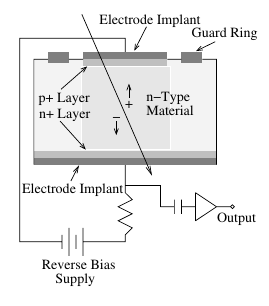
\includegraphics[width=0.4\textwidth]{03_Prototype/figures/fig000_Si_detector.png}
	\caption[Principle of a simple semiconductor detector]{Principle of a simple semiconductor detector\cite{Ahmed2007}.}
	\label{chap3:}
\end{wrapfigure}

  When highly doped $p$ and $n$ semiconductors are put in contact, the charge concentration of both carriers presents an important gradient at the interface, known as depletion region. Therefore, the electrons move to the $p$ doped region, leading to an electric field which blocks the electron flows. Thereafter, the junction is at equilibrium. In reverse bias mode, a positive potential is applied between $n$ and $p$ regions, then the depletion zone becomes bigger and the capacitance of the junction decreases. When a charged particle passes through the silicon detector, it deposits its energy and electron/hole pairs are created as described in the section \ref{chap3:sec_particle_in_matter} of this chapter. The charge carriers drift in the semiconductor due to the bias voltage, inducing a signal on electrodes as described by the Ramo-Shokley theorem, also valid for semiconductors.\cite{Cavalleri1971}.
  \begin{equation}
    i(t) =  \boldsymbol{E_{wpixel}} \left( q_{electron} v_{electron}  + q_{hole} v_{hole} \right)
  \end{equation}
  where $\boldsymbol{E_{wpixel}}$ is the weighting field of a pixel pad, $\boldsymbol{E_{bias}}$ is the field due to $V_{bias}$, $v$ is the speed of the charge carriers and $q$ their charges. Table \ref{chap3:semiconductor} lists the properties of common semiconductors used in radiation detection.
  \begin{table}[!ht]
	\centering
	\caption[]{Properties of common semiconductors \cite{NSM2005,Eisen1996} used as radiation detector. Properties are given at NTP conditions.}
	\label{chap3:semiconductor}
	\begin{tabularx}{\linewidth}{lXXX}
    \toprule
    Property & $Si$ & $Ge$ & $CdTeZn$ \\
    \midrule
    Density ($\mathrm{g/cm^3}$)& $2.33$  & $5.32$ & $5.78$ \\
    $W$ value ($\mathrm{eV}$) & $3.6$ & $2.95$ & $4.64$ \\
    Breakdown ($\mathrm{V/m}$) & $\approx 3\cdot10^5$ & $\approx 10^5$ & $\approx 10^5$\\
    $e^{-}$ mobility ($\mathrm{cm^{2}/V/s}$) & $\leq 1400$ & $\leq 3900$ & $\leq 1100$\\
    $h$ mobility ($\mathrm{cm^{2}/V/s}$) & $\leq 450$ & $\leq 1900$ & $\leq 100$ \\
    Usage & General purpose & $\gamma$-ray & $X$-ray\\
    Cost & Cheap & Expensive & Moderate\\
		\bottomrule
	\end{tabularx}
\end{table}


  In monolithic sensors, the detection and the electronic functions are integrated together in the same substrate. These sensors achieve very small dimensions due to their high level of integration. Usually, monolithic sensors are developed for a specific purpose and are produced in large quantity reducing the costs.

  In hybrid pixel detectors, detection and readout functions are physically separated. The detection matrix is placed on the readout electronics and the connection between the pads and the readout circuits is ensured by bumps. The reading system is independent of the detection matrix making this technology more generic and accessible for small volumes.

  Semiconductor sensors could be interesting as readout system for the \acrshort{ipm}s. An electron of $15\,\mathrm{keV}$ deposits all its energy and creates a few thousand of electron/hole pairs in the sensitive silicon layer. Unlike strips or \acrshort{mcp}s the energy of the incident particle is recovered, enabling background discrimination. At last, electronic dead times are typically in the ns to µs range.

  On the other hand, the use of semiconductor with ions at low energies ($< 30 \,\mathrm{keV}$) is uncertain. Indeed, an aluminium coating is often deposited on the top of the sensor for insuring a correct polarization and the superficial layer of the sensor are not active, which represents about a hundred nm dead zone. As shown in Fig. \ref{chap3:ion_si_deposit}, $H_{2}^{+}$ ions loose $15\,\mathrm{keV}$ in $200\,\mathrm{nm}$ silicon layer, meaning that most of the electron/hole pairs are created and deposited before reaching the sensitive layer.

  Low energetic ions may also produce more damages than electrons in the semiconductor lattice. The creation of charge traps and the depletion zone modifications are the worst damage scenarios. Modern semiconductors often implement a pixel calibration circuit to compensate non uniformities.

  \subsection{MCP based detection}

  A MicroChannel Plate (MCP) generates electrons from incident ionizing particles \cite{Wiza1979}.
  It can be seen as a glass lead plate drilled with micro-metric tilted holes.
  A specific coating is applied on its input surface to increase secondary emissions. When a particle hits the \acrshort{mcp} hole entrance, secondary electrons are emitted. Due to the difference of potential applied between the \acrshort{mcp} faces, secondaries are drawn towards the channel output and strike hole walls again, creating more and more electrons. Then, electrons are collected on a detection plane that can be a single electrode, multiple electrodes or a phosphorus screen depending on the read-out requirements. Fig. \ref{chap3:MCP_outline_1} shows some schematic representations of how an \acrshort{mcp} works.

  \acrshort{mcp}s have a high efficiency for low energy ions and electrons. \acrshort{mcp}s are also sensitive to photons via compton and photoelectric effect interactions (from gamma rays to VUV). The detection of neutron is  also possible by adapting the composition of the coating. \acrshort{mcp}s are fully vacuum compatible. \acrshort{mcp}s are also extremely fast amplifiers and time resolution is in the order of a few hundred picoseconds for a single stage \acrshort{mcp}. The spatial resolutions of a \acrshort{mcp} depends on its channel size and spacing. However both resolutions are limited by the readout used. Phosphorus screens provide high spatial resolution but screen are not fast as the \acrshort{mcp}. Electrode readout allows to read fast and low signals with an efficient electronic.

  \begin{figure}[!ht]
	\begin{center}
		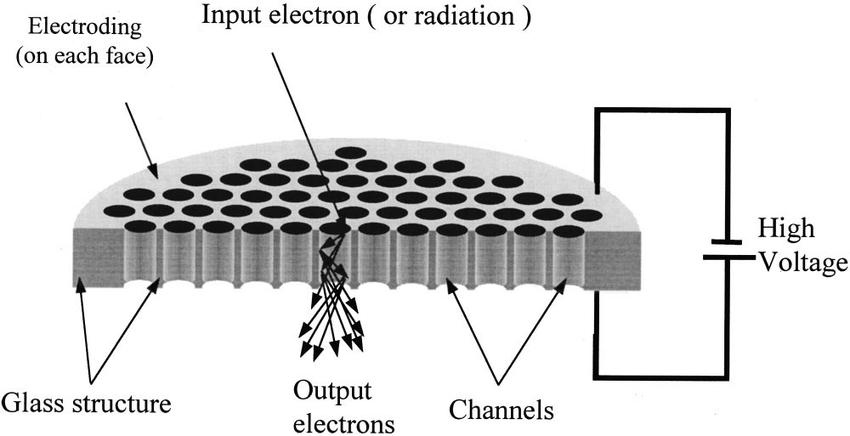
\includegraphics[width=0.7\textwidth]{03_Prototype/figures/fig031_MCP_outline}
	\end{center}
	\caption[]{Sectional view of a MCP \cite{Yi2001}.}
	\label{chap3:MCP_outline_1}
\end{figure}


  The gain or multiplication factor for a single \acrshort{mcp} is about $10^{2}$ to $10^{4}$ depending on the $V_{MCP}$ voltage, usually from $600$ to $1000\,\mathrm{V}$. Several \acrshort{mcp}s can be stacked to increase the gain to $10^{6}$ or even higher. Typical configurations are single stage, chevron stack (double stages) or Z stack (triple stages). Obtaining an analytical expression of the gain is not trivial since it strongly depends on the characteristics of the \acrshort{mcp} and its coating. \acrshort{mcp} manufacturers often express the gain as an exponential function of the potential applied.

  \begin{figure}[!ht]
	\begin{subfigure}[t]{0.5\textwidth}
		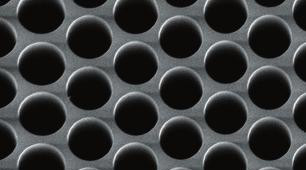
\includegraphics[width=\textwidth]{03_Prototype/figures/fig030_MCPoutline_b2.jpeg}
		\caption[SEM picture of MCP holes]{SEM picture of MCP holes \cite{HamamatsuMCP}.}
		\label{chap3:MCPholes}
	\end{subfigure}
	~
	\begin{subfigure}[t]{0.5\textwidth}
		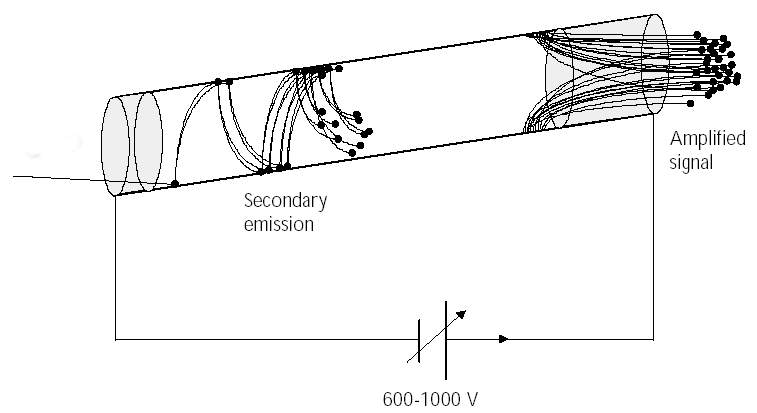
\includegraphics[width=\textwidth]{03_Prototype/figures/fig030_MCPoutline_a.png}
		\caption{Description of how an MCP amplifies incident particle.}
		\label{chap3:MCPchannel}
	\end{subfigure}
	\caption[Schematic views of how a MCP works]{Schematic views of how a MCP works.}
	\label{chap3:MCPoutline}
\end{figure}


  Unfortunately \acrshort{mcp}s have some drawbacks, the first one being ageing. Indeed the coating is damaged by the incident particles, thus the gain is not stable and decreases over the time. A second disadvantage is the \acrshort{mcp} gain limitation due to saturation. If the incident particle flux is too high, holes may be saturated, and they cannot amplify anymore. When this happens to a channel, it takes some time to recover, generating dead time.

  %\section{Background signal }
  %\subsection{Background from beam particles }
  %\subsection{Secondary emission }

  \section{Summary}
  \label{ch3:Summary}
  This chapter exposed all the studies that have been performed to prove the feasibility of an \acrshort{ipm} for the cold part of the \acrshort{ess} accelerator. Three key points were identified: the number of ionization particles, the distortion on the profile and the choice of the readout system.

  The \acrshort{ess} conditions are particularly unfavorable for the ionization cross sections since the high vacuum level in the accelerator does not help. Direct calculations and simulations show that the order of magnitude of the number of ionization particles is about a few thousand particles per pulse per cm for nominal \acrshort{ess} conditions. This number of primary particles seems sufficient to perform a profile measurement assuming that these particles may be detected by the readout.

  The non-uniformity of the electric field can be corrected effectively using field correctors and shielding disks regardless of the configuration used. However the symmetrical mode is easier to correct and reduces the maximum voltage required.

  The simulations clearly show that the ions are less sensitive to the phenomenon of space charge. The profile measurement with electrons introduces an error that does not fulfil the \acrshort{ess} requirements, since it is impossible to install a correction magnet to constrain the trajectories of the electrons. Therefore the measurement of the profile will be done in ions configuration.

  The use of ions complicates the choice of the readout. Strips are an extremely robust method but it requires a low noise electronics. \acrshort{mcp}s amplify the signal but these devices suffer of aging effect. Silicon detectors are very promising because they are very sensitive, resistant and fast. However, the detection of low energetic ions with these detector is not assured and their implementations are quite complex.

  All of these studies were presented during a Preliminary Design Review (January 2017) which marked the beginning of the construction phase of the different prototypes.

  \cleardoublepage
  \section*{Bibliography}
  \addcontentsline{toc}{section}{Bibliography}
  \label{ch3:bib}
  \printbibliography[heading=subbibliography]

\end{refsection}
